%
% phd-summary
%
% Licensed under none License
%

% Page creation engine
\documentclass[11pt,a4paper]{book}
\usepackage[utf8]{inputenc}
\usepackage[french]{babel}
\usepackage[T1]{fontenc}

% Main modules
\usepackage{url}      % URL
\usepackage{graphicx} % Pictures
\usepackage{wrapfig}  % In-line Pictures
\usepackage{verbatim} % Code
\usepackage{mathtools,amssymb}
\usepackage{minted}   % Code
\usepackage{xcolor}   % Color text
\usepackage{textgreek}% Greek language
\usepackage{booktabs} % Tables
\usepackage{colortbl} % For coloring rows, columns of table
\usepackage[toc,page]{appendix} % For managing appendix sections cleanly
\usepackage{algpseudocode} % For displaying pseudo-code
\usepackage{amsmath,empheq} % Math equations
\usepackage[nomain,acronym,xindy,toc]{glossaries}
\usepackage{makeidx}  % index support
\usepackage{caption}     % float env with page breaks
\usepackage{hyperref}    % Links

\pagestyle{myheadings}

% Meta-data
\title{}
\author{ \\ }
\date{Résumé en français}
% Glossary
\loadglsentries[main]{../src/glos}
\makeglossaries
\makeindex

% Document
\begin{document}

\begin{titlepage}
	\centering
	{\scshape NXP Semiconductors \par}
	\vspace{0.5cm}
  {\scshape ET \par}
	\vspace{0.5cm}
  {\scshape LAAS-CNRS (Laboratoire d'Analyse et d'Architecture des Systèmes) \par}
  \vspace{1cm}
	{\scshape\Large Thèse CIFRE - Résumé en Français\par}
	\vspace{1.5cm}
	{\huge\bfseries Développement de méthodes d'analyse hiérarchique des défauts fonctionnels liés aux décharges électrostatiques pour les circuits intégrés analogiques\par}
	\vspace{2cm}
	{\Large\itshape Rémi Bèges\par}
	\vfill
	supervisé par\par
	Dr. Fabrice \textsc{Caignet} (LAAS-CNRS)\par
  Dr. Patrice \textsc{Besse} (NXP)\par
  Pr. Marise \textsc{Bafleur} (LAAS-CNRS)\par

	\vfill

% Bottom of the page
\end{titlepage}

% Chapter files listing
\chapter{Introduction}

% Trends of the electronic field is size reduction
La miniaturization des circuits électroniques se poursuit malgré des barrières technologiques de plus en plus élevées.
La diminution de taille des circuits intégrés permet une réduction des coûts grâce à l'augmentation des volumes de production.
La réduction de poids des modules électroniques pour l'automobile ou l'aéronautique permet des réductions de carburant, de coût, et moins d'impact sur l'environnement.
A taille constante, des circuit intégrés plus denses peuvent embarquer plus de fonctionnalités et ont des performances plus élevées.

% How is size reduced
La réduction de taille des circuits intégrés est possible en utilisant des technologies silicium plus fines.
Une technologie silicium définie les dimensions et les formes d'un ensemble de briques de conception électronique, formant une librairie de composants, ainsi que tous les procédés nécessaires à la fabrication du circuit intégré.
La plupart du temps, ces librairies de composant sont constituées de différents types de transistors, diode, résistances et capacitances.
La taille d'une technologie est définie par la plus petite dimension possible pour une grille de transistor, aussi appellée \textlambda.
La valeur de \textlambda est essentielle et conditionne fortement la taille du circuit final, sa consommation et ses performances.
Jusqu'à présent, la loi de Moore a prédit avec succès que \textlambda serait réduit d'un facteur deux tous les dix-huit mois.
Le domaine automobile se conforme à cette tendance, en utilisant récemment des noeuds technologiques à 16nm (Fig. \ref{fig:nxp-techno-increase}) \cite{evolution_technologies} normalement utilisés dans des applications moins sévères.

\begin{figure}[!h]
  \centering
  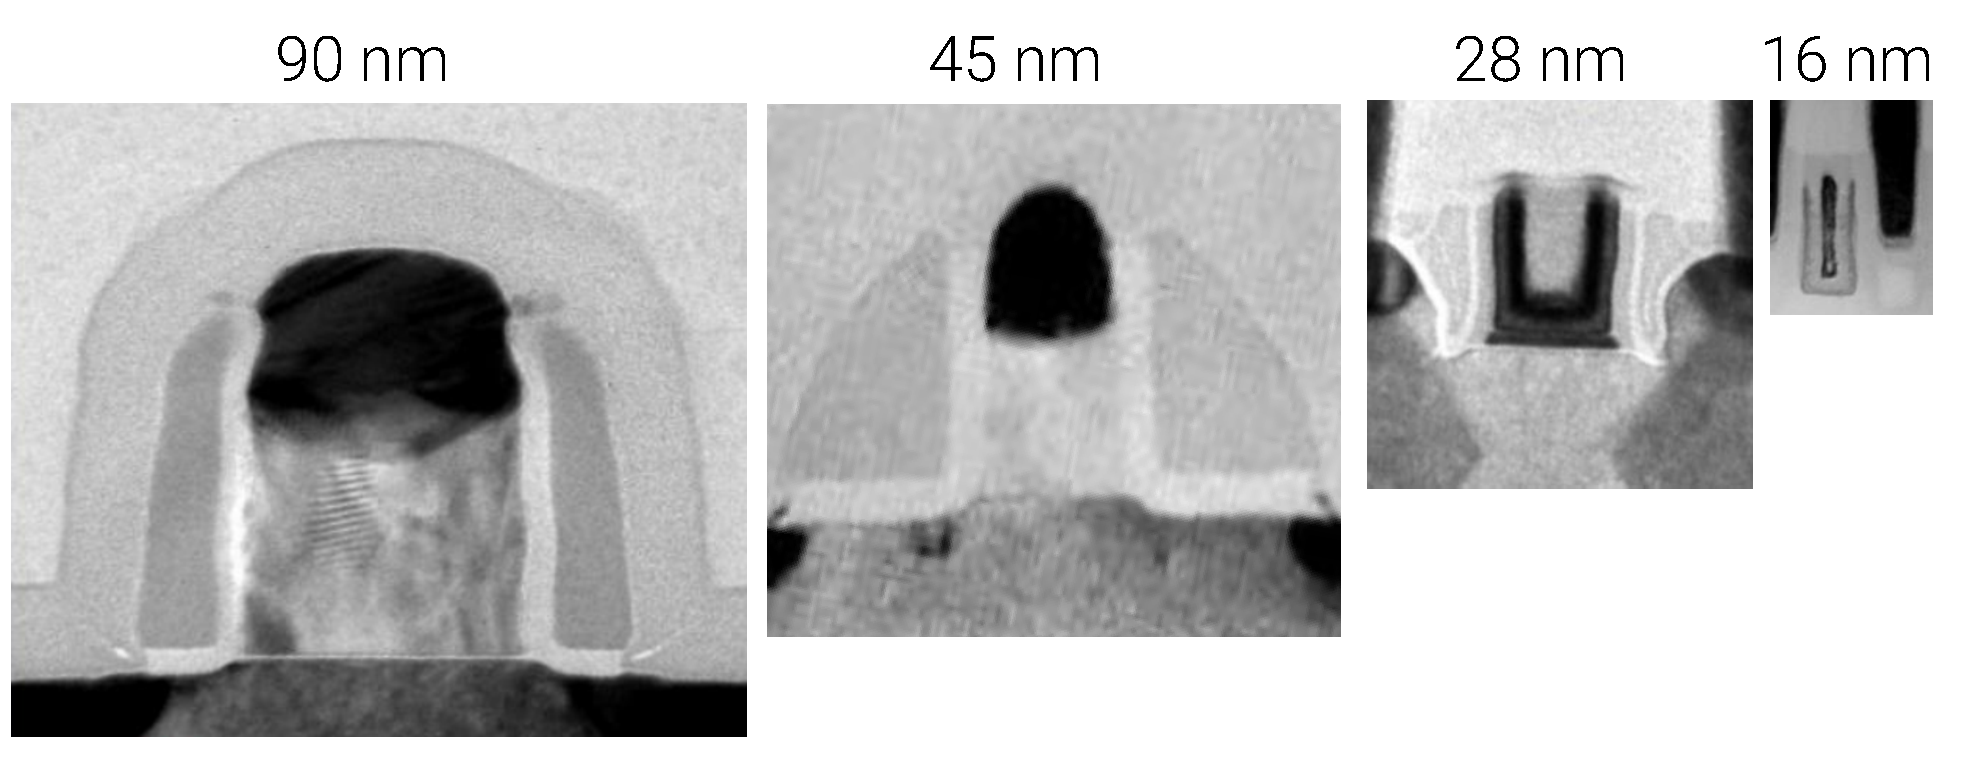
\includegraphics[width=\textwidth]{src/1/figures/technology_evolution.pdf}
  \caption{Recent evolution of NXP's automotive technology nodes \cite{evolution_technologies}}
  \label{fig:nxp-techno-increase}
\end{figure}

% Side effects of size reduction
Cette réduction de taille s'accompagne d'une augmentation de la fragilité et de la sensibilité des circuits intégrés.
Les seuils de tolérances en tension et courant deviennent plus petits, au delà desquels les circuits sont détruits.
La surface de silicium nécessaire à la protection des coeurs de circuits occupe une plus large part de l'aire totale d'un produit  \cite{evolution_technologies}, et donc du coût.

% Another trend in automotive - more electronic functions
De nos jours, de nouvelles fonctionnalités majeures sont aussi en dévelopement dans le domaine automobile.
En particulier, les véhicules autonomes ou l'aide à la conduite font leur apparition sur les routes.
Ces fonctionnalités font en permanence des décisions et prennent des actions critiques sur le véhicule, comme tourner le volant ou enclencher le freinage.
Elles sont implémentées afin d'augmenter la sécurité des usagers d'un véhicule, ce qui résulte en des responsabilités et des contraintes accrues sur les modules électroniques.
La sûreté de fonctionnement des ces modules est donc vitale pour ce type d'application.

% Another trend is reduced power consumptions
L'augmentation de la quantité d'électronique dans un véhicule s'accompagne aussi d'une forte hausse de la consommation électrique.
Au niveau circuit-intégré, les tensions d'alimentations sont réduites très bas, avec communément des seuils d'alimentions de 1V.
Les marges de bruit des cellules digitales sont réduites d'autant, rendant les circuits bien plus sensibles aux perturbations électriques.

% Harsh environment in the automotive field
Par ailleurs, l'environnement automobile est très sévère pour les composants électroniques.
Un moteur en fonctionnement génère de la chaleur et des vibrations.
Durant toute sa vie, un véhicule est exposé à de larges cycles thermiques.
Les contacts électriques, les soudures et les connections vieillissent plus rapidement à cause de cela.
De plus, les systèmes électroniques sont exposés à une large plage de stress électriques.
Quand le moteur est allumé, la tension de batterie chute fortement à cause de l'appel de courant créé par le démarreur.
Cette variation très brutale peut affecter ou endommager les modules.
Il existe également une autre famille de perturbations électriques appellée décharges électrostatiques, et produite par l'environnement du véhicule.

% What is an ESD
Une décharge électrostatique est un transfert de charge soudain entre deux objets de différente charge.
C'est le résultat d'une accumulation de potentiel électrostatique.
La décharge se produit lorsque la différence de potentiel est suffisamment large.
L'amplitude de tels événements peut atteindre couramment plusieurs milliers de volts et des dizaines d'ampères.
Le fabricant de véhicules Renault estimes que les composants électroniques automobiles sont exposés 10000 fois à des décharges pendant leur vie \cite{Renault-esd}.

% Architecture systemes automobiles
L'architecture des systèmes électriques dans un véhicule est également très complexe et rude pour les modules électroniques.
Une voiture est consistutées d'une multitude de modules électroniques interconnectés par des câbles.
C'est un vrai challenge pour garantir la robustesse de cet ensemble contre des perturbations électriques.
La seule connection d'une voiture à une vrai référence électrique se fait par les pneus, ce qui équivaut globalement à une très mauvaise connection à la terre.
Néanmoins, les modules électroniques ont besoin d'une bonne référence pour communiquer entre eux et fonctionner correctement.
Ceci est assuré par la carcasse métallique du véhicule.
En statique et à basse fréquence, cette référence est très bonne car très peu résistive.
Les décharges électrostatiques sont au contraire des évènements avec la majorité du spectre à très haute fréquence, jusqu'à 1 GHz environ.
Dans cette gamme de fréquence, la carcasse métallique ne se comporte plus comme une bonne référence et les cables deviennent largement inductifs.
Ces phénomènes peuvent donc fortement perturber les systèmes électroniques.
De plus, les cables peuvent rayonner et les propagations peuvent se propager par couplage.
Globalement, l'architecture d'un véhicule est complex et sensible par nature aux perturbations.

\begin{figure}[!h]
  \centering
  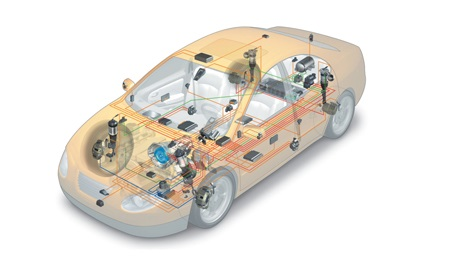
\includegraphics[width=0.6\textwidth]{src/1/figures/systemintegration_01_uv-data.jpg}
  \caption{Architecture of electronic systems in a vehicle \cite{car-architecture}}
  \label{fig:car-architecture}
\end{figure}

% Fiabilite vis a vis des ESD
En résumé, la quantité de composants électroniques est en augmentation et en parallele ils deviennent de plus en plus sensibles.
De plus, ils doivent opérer dans une environnement électrique sévère, avec de multiples sources de perturbation.
Ces perturbations peuvent créer des défaillances.
Dans le domaine des décharges électrostatiques, il y a deux types de défaillances à considérer.
La casse matérielle est le résultat de la destruction permanente d'un composant.
Les circuits intégrés sont particulièrement vulnérables \cite{impactESDsemiconductors} et nécessitent des mesures de protection.
Récemment, un deuxième type de défaillance commence à être étudié.
Les défaillances fonctionnelles sont une perturbation d'une fonction électrique du circuit intégré à la suite d'une décharge.
Plusieurs niveaux de sévérité existent.
La perturbation du système d'airbag est par exemple bien plus critique celle du système de tableau de bord.

\begin{figure}[!h]
  \centering
  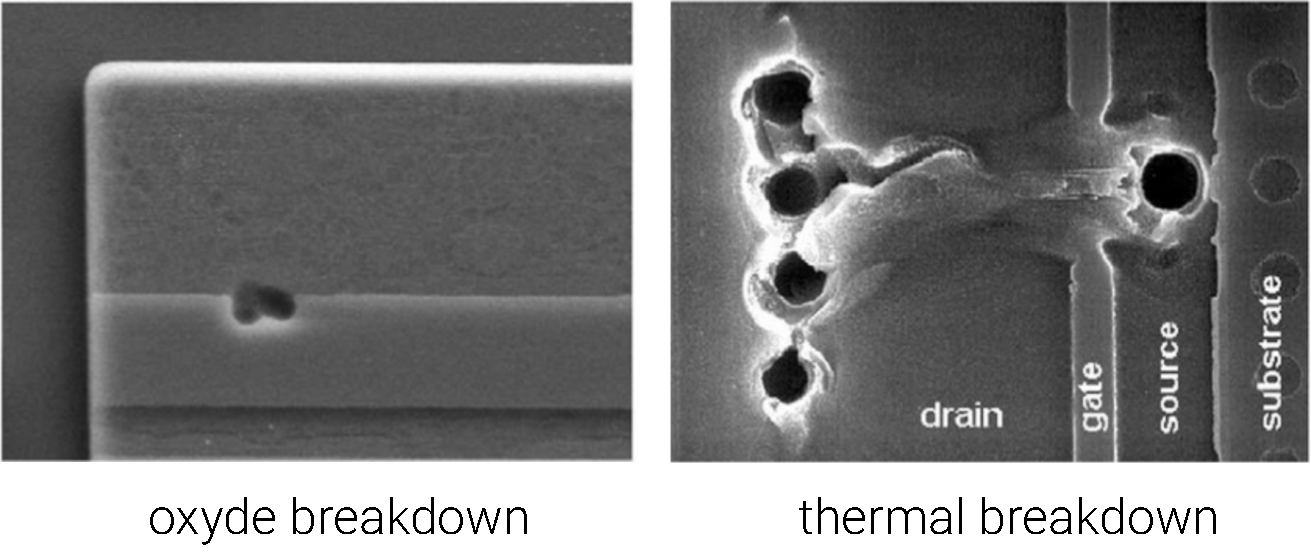
\includegraphics[width=0.4\textwidth]{src/1/figures/esd_failures.jpg}
  \caption{Different kinds of ESD-induced failures}
  \label{fig:esd-failures}
\end{figure}

% Comment predire ces defaillances fonctionnelles
Des travaux sur ce sujet ont été publiés par F. Caignet et N. Lacrampe en 2007 \cite{}.
Egalement, de nombreuses recherches sur les défaillances au niveau système ont été publiées pendant les symposia EOS/ESD 2012 \cite{} et 2013 \cite{}.
De plus, le standard IEC 62433-6 encore en phase d'élaboration cherche à formaliser des méthodes de base pour l'analyse et la prédiction de faiblesses fonctionnelles.
Globalement, les recherches dans ce domaine restent focalisées au niveau système.
Dans ce document, la recherche et l'analyse de faiblesses fonctionnelles a lieu plus bas dans la hiérarchie, au niveau circuit-intégré.

% Presentation des chapitres
%
Le chapitre \ref{chap:1} fournit en détail les notions essentielles à la compréhension de la problématique.
Il explique comment les décharges électrostatiques apparaissent et comment elles sont reproduites en laboratoire.
Ensuite, une revue de l'état de l'art est présentée sur l'analyse des pertes de fonctionnalités dues à des décharges.

%
La chapitre \ref{chap:2} présente un méthode de modélisation pour simuler la propagation de décharges électrostatiques jusqu'au composant.
C'est une part important du problème que d'identifier quelle fraction d'une décharge atteint réellement un circuit intégré.
Une librairie de modèles est construite, ensuite assemblés ensemble pour reproduire le système à simuler.
Un générateur de stress utilisé dans le laboratoire de test à NXP est modélisé pour illustrer la méthode.
Un nouveau générateur de stress, appellé TLP-HMM est ensuite proposé, reproduisant une forme d'onde standardizée mais avec des avantages importants sur les générateurs actuels.
Ce générateur est particulièrement intéressant pour effectuer des tests de décharge sur circuits intégrés.

%
Un cas de défaillance fonctionnelle est ensuite présenté dans le chapitre \ref{chap:3}.
Tout d'abord, des mesures sont effectuées de manière externe sur le circuit intégré sous test.
La signature de la défaillance est expliquée.
Ensuite, un circuit intégré de test est développé et fabriqué sur silicium.
Il contient des structures spéciales pour mesurer les pertubations directement depuis le silicium.

%
Ces travaux ont aussi été orientés vers la recherche de nouvelles méthodes de simulation.
L'objectif est de détecter plus facilement et rapidement des défaillances fonctionnelles, en utilisant les outils existants de simulation.
Trois méthodes différentes sont présentées dans le chapitre \ref{chap:4}.
Elles ont chacune des applications différentes, mais peuvent s'avérer complémentaires pour concevoir des circuits robustes.

%
Enfin, la conclusion résume les travaux effectués et présente des axes de recherche futurs.

\chapter{Tests et analyse défauts fonctionnels ESD}
\label{chap:1}
\section{Contexte}

% What is an ESD, its key properties
An electrostatic discharge (ESD) is the result of the accumulation of electrostatic potential.
It is a very sudden current flow that propagates through metallic or non-metallic materials, electrical systems and sometimes even through the air.
It is a very short electrical event, involving large currents and extremely high voltages.
\gls{ESD} have durations in the range of a few hundred nanoseconds.
Currents can reach tens of amperes and voltage levels several thousand of volts.
The total discharge energy is small, somewhere near the milli-Joule (mJ).
The power on the other hand is extremely high because the waveforms are changing extremely rapidly.

% What generates an ESD
Objects can accumulate electrostatic potential by tribocharging or electrostatic induction.
In the case of tribocharging, electrons are transferred from one object the other when they are put into contact then separated.
One object becomes positively charged and the other negatively.
Which object gains electrons depends on the kind of material constituting each object.

% Electronic devices are exposed to ESD, in factories first
As detailed in the introduction, electrostatic discharges constitute a large threat for electronic devices.
Failures can occur during manufacturing and or normal operation.
The manipulation of parts by manufacturing machines involves repeated contact and separation.
Ultimately, triboelectrification and discharges happen and devices can get destroyed.
Several standards exist to guarantee that devices can survive this manufacturing step.

Parler HMM, MM, CDM
Tests for manufacturing env

% Electronic devices are exposed to ESD in the field
After manufacturing, failures can happen with the device in the field and exposed to its operating environment.
Manipulation by electrically-charged humans is a major source of danger for commercial products like cellphones and cameras.
The automotive environment is even harsher, with vehicles being a major source of electrostatic discharges.

% Hard-failure is one thing, soft-fail another
Integrated circuits are studied and protected against hard-failure since a few decades.
Despite this experience of the \gls{esd} community, it remains challenging to perfectly protect an electronic system against hard-failures.
Nowadays, a new class of failures appears.
Instead of studying permanent failures, devices are studied for temporary failures affecting their functionality.
These are called soft-failures or functional failures.
\gls{esd} can cause them to happen, with diverse consequences.
In less severe situations, functionnality of a chip is disturbed just for the duration of the ESD and recovers immediately without noticeable consequence.
The failure remains located inside the integrated circuit and does not impact the application above.
Sometimes, the discharge is harmful enough to cause a circuit to restart because the \gls{esd} disturbed some critial nets or parameters.
This is common when supply voltages go out of specification for instance.
Startups or power-on reset functions understands overvoltage or undervoltage as the signal for a regular power-up sequence.
The device can also perform restarts to try a recovery because proper operations cannot be guaranteed, due to unexpected values on some nets.
Most microcontrollers for instance monitor supply voltages of digital gates.
If the voltage is too low, the noise margins of the gates cannot be guaranteed and proper operations either.
At this point, the microcontroller restarts to try to recover.
Restarts are slow processes compared to the operation of a chip.
For critical applications, this delay is highly unwanted because it impacts human safety.
The availability of the chip that triggers airbags in a car is vital for instance.
In a more severe scenario, the system gets completely frozen or stuck into an unwanted state because of the \gls{esd}.
The only way to recover normal operation requires a user-intervention.
User intervention can take the form of turning the key to shut down and restart the vehicle's engine.
Finally, hard-failure can be seen as the next step immediately after the most severe soft-failure.
The device is in a non-recoverable state and must be replaced.
Hard-failures are not considered for functional robustness analysis.

\section{Méthodes de test ESD}

To reproduce disturbances in lab, multiple stress generators

% History of TLP
The transmission line pulsing generator is an extremely popular tool in the \gls{esd} field.
Over the years, it was employed in a variety of applications, from characterization of devices \cite{TLPforESDProtectionCz, TLPthroubleshooting}, investigation of failures \cite{tlp-application-1, tlp-application-2} and correlation of failure levels with other generators \cite{correlation-system-level-esd-tlp}.
It is a versatile tool, that was often modified to adress larger testing conditions \cite{tlp-power} or non-rectangular pulse waveforms \cite{tlp-based-hmm, my-publi-tlp-hmm}.
The technique was invented by T. Maloney and N. Nakamura \cite{TLP}.
It is in the process of standardization as part of ANSI/ESD STM 5.5.1-2016 \cite{tlp-standard} through the effort of the ESD Association (ESDA) \cite{esda}.
It was extensively studied during the PhD thesis of N. Monnereau \cite{phd-monnereau} and N. Lacrampe \cite{phd-lacrampe}.

% Concept
\gls{tlp} systems produce a short rectangular pulse, through the discharge of a coaxial cable (Fig. \ref{tlp_concept}).
The cable is initially charged with an high-voltage voltage supply through a high value resistor.
This keeps the current small and avoids oscillations on the cable.
When the voltage of the cable reaches the desired amplitude, a relay can be switched to trigger the discharge.
The coaxial cable has usually a characteristic impedance of 50\textOmega{} and a length of 5 metres, corresponding to a 50ns propagation delay.
The generated pulse is twice that delay.

\begin{figure}[!h]
  \centering
  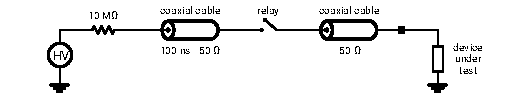
\includegraphics[width=\textwidth]{src/1/figures/tlp_concept.pdf}
  \caption{Minimal example of a \gls{tlp} system}
  \label{tlp_concept}
\end{figure}

% Characteristics of tlp systems
TLP systems constitute very well-controlled test generators.
The pulse is generated inside a shielded environment.
It is isolated from external radiated emissions and does not emit electromagnetic disturbances.
The characteristic impedance of 50\textOmega{} can be controlled up to the load, by using appropriate 50\textOmega{} cables and hardware.
Those properties result in clean and repeatable pulse waveforms without reflections.
The main features of the generated pulse are given in figure \ref{tlp_pulse}.

\begin{figure}[!h]
  \centering
  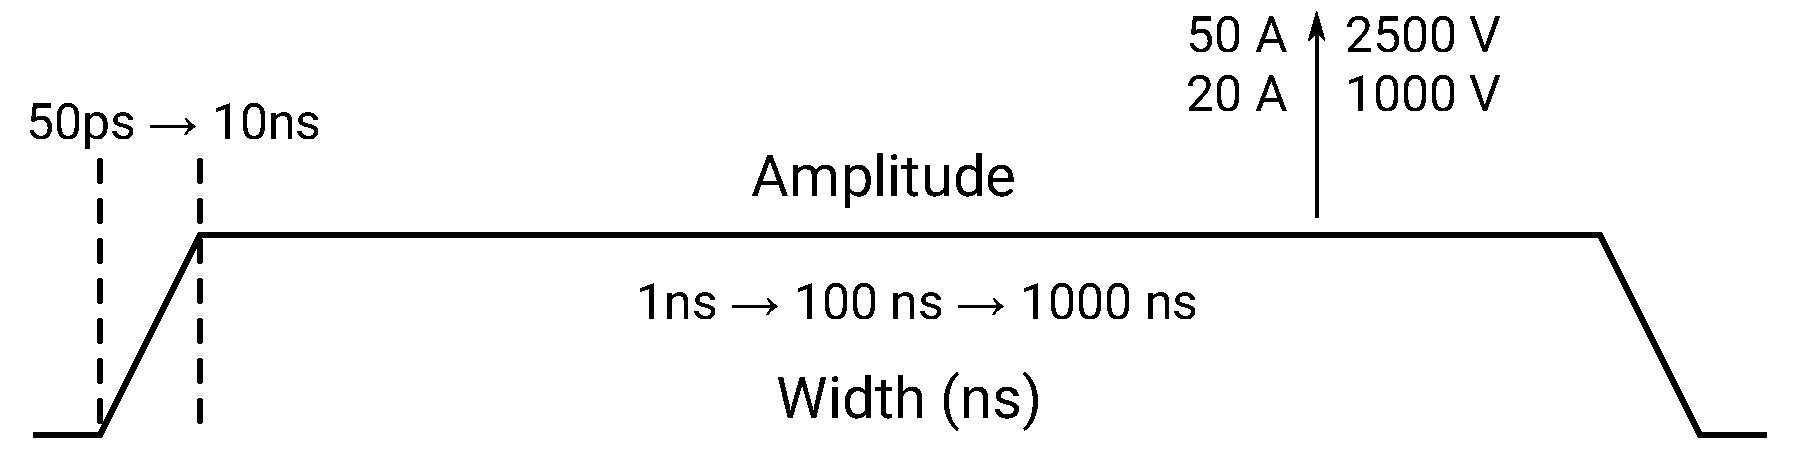
\includegraphics[width=\textwidth]{src/1/figures/tlp_pulse.pdf}
  \caption{Main characteristics of a \gls{tlp} pulse on a resistive load}
  \label{tlp_pulse}
\end{figure}


Pistolets de décharge ESD

% What is the goal of this test
IEC 61000-4-2 \cite{iec61000-4-2} and ISO 10605 \cite{iso10605} standards define a system-level test waveform and test generator to reproduce the discharge of a human body through an electronic device.
This test is used very extensively for qualification of products.
Fig. \ref{fig:picture-esd-gun} provides a picture of an \gls{esd} gun.
The gun is composed of a metallic discharge tip to inject the pulse.
The ground return is a long metallic ribbon a couple of meters long.
Depending on the test configuration, it is connected to the product ground or the earth.
Its shape impacts a lot recorded failure levels.
Historically, ESD gun were famous for lacking some reproducibility on test results \cite{hmm-uncertainty}.
They have largely improved since then although radiated emissions and shape of the ground return still remain a very large factor of variation and uncertainty \cite{gun-rf-uncertainty}.

% How is the pulse generated
The generation of the ESD pulse is done with a 330\textOmega resistor and 150 pF capacitor discharge network.
The RC network alone though does not suffice to reproduce the waveform.
Parasitic devices play an important part in shaping the waveform.
Fig. \ref{fig:esd-gun-model} provides a physically-based ESD Gun model that helps understand the impact of parasitic devices.
This model was originally written by Chiu \cite{phd-chiu} and is referenced in the PhD thesis of N. Monnereau \cite{phd-monnereau}.
It adds an R\textsubscript{g}L\textsubscript{g}C\textsubscript{g} network to model the ground return.
A parasitic capacitance C\textsubscript{i} and series inductance L\textsubscript{i} model imperfections in the direct injection path.

\begin{figure}[!h]
  \centering
  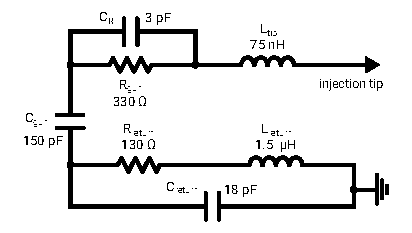
\includegraphics[width=0.3\textwidth]{src/1/figures/gun_model.pdf}
  \caption{ESD Gun model}
  \label{fig:esd-gun-model}
\end{figure}

% Explain the waveform
%TODO: Why 2 ohms ?
Fig. \ref{iec_pulse} presents the main properties of the generated stress.
The standard defines this waveform for a 2\textOmega{} load.
The pulse starts by a fast peak with a $1ns$ risetime.
It is followed by a slower slope of smaller amplitude but longer duration of about $200ns$.
Voltage levels can reach 15kV peak and 30A of current.

\begin{figure}[!h]
  \centering
  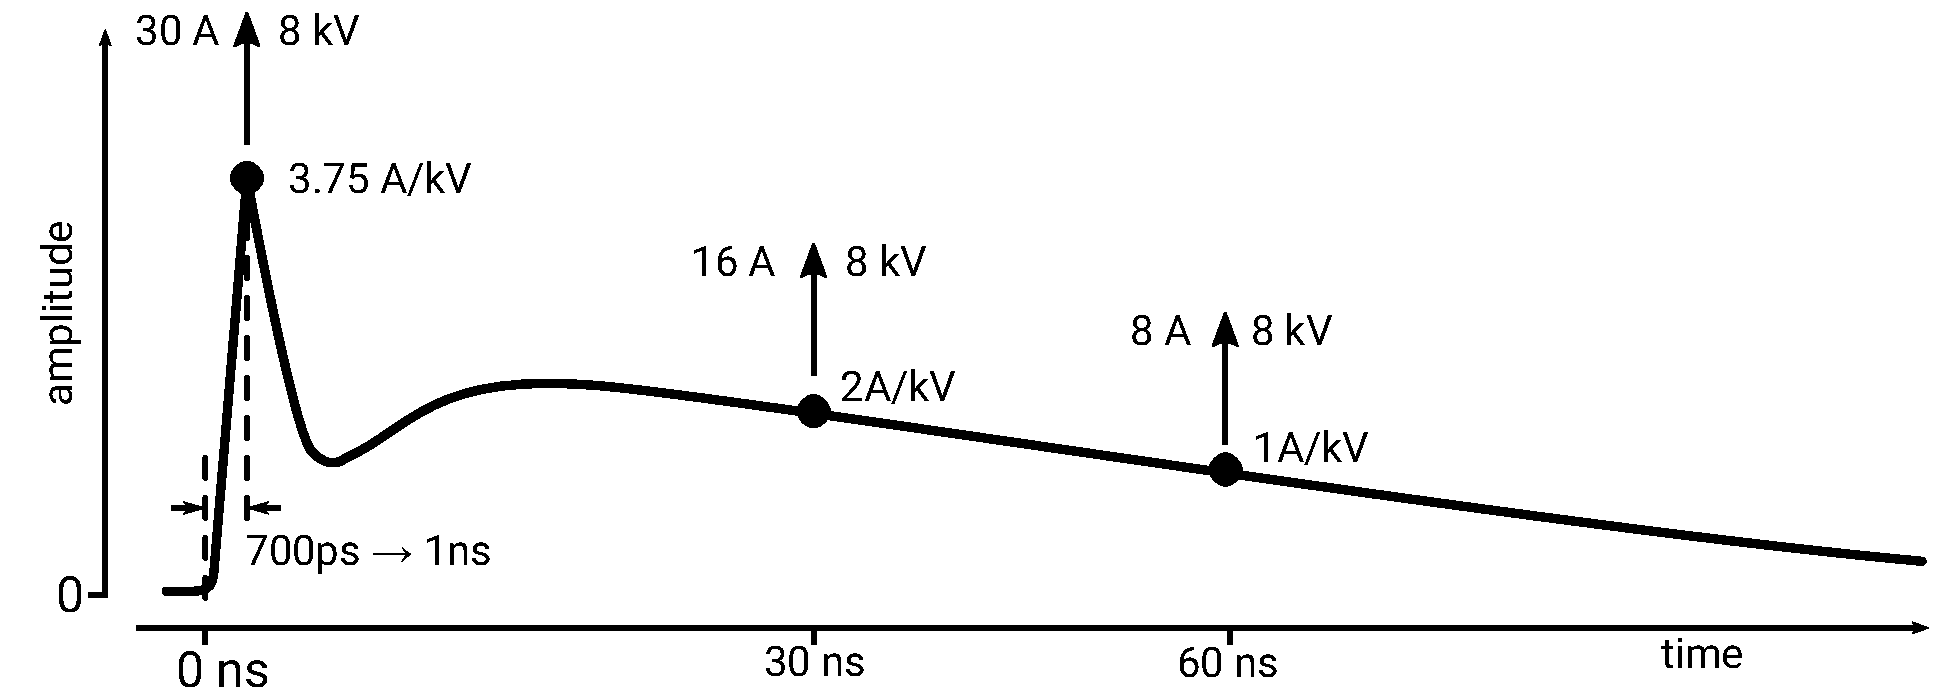
\includegraphics[width=\textwidth]{src/1/figures/iec61000-4-2_waveform.pdf}
  \caption{Main properties of an IEC 61000-4-2 pulse on a 2\textOmega\ resistive load}
  \label{iec_pulse}
\end{figure}

Other test methods exist, such as ... Test automobile ISO, Méthode DPI standardizée

\section{Méthodes d'analyse de faiblesses fonctionnelles}

% Case 1 - NXP bandgap + substrate coupling
K. Abouda details in \cite{softfailEMCIC} a case of soft-failure on an integrated automotive regulator \gls{ic}.
The failure signature is a loss of the regulated voltage when exposed to \gls{bci} ISO11452-4 \cite{iso11452}.
The test setup is provided in Fig. \ref{}.
The product is investigated manually, by searching inside the design for coupling and propagation paths, and performing multiple simulations.
Eventually, it was proven that a residue of the disturbance was coupling through the substrate on a current mirror inside the bandgap reference.
During the disturbance, bandgap voltage was shifting from its nominal value.
After some delay, the bandgap output was reaching an undervoltage threshold, causing the entire system to restart.
To avoid it, a design fix was proposed by filtering at the appropriate spot inside the design to avoid the amplification of the disturbance.

\begin{figure}[!h]
  \centering
  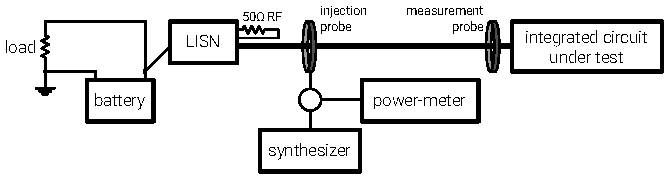
\includegraphics[width=\textwidth]{src/1/figures/bci_setup.pdf}
  \caption{Bulk Current Injection setup}
  \label{fig:bci-setup}
\end{figure}

% Case 2 - CESAME IC - paper Vrignon + Ben dhia
N. Lacrampe presents another failure case in \cite{LacrampeTransientImmunity}.
Very-fast \gls{tlp} is injected on an 0.18 \textmu{}m CMOS technology (1.8 V supply voltage) testchip.
The chip contains 6 instances on the same logic core, differing only by their power-rails architecture.
The injection on power rails is performed using a \gls{dc} block 1 nF capacitor, similarly to the \gls{dpi} standard \cite{iec62132-4}.
% What is the failure signature
An output signal of the logic core is monitored.
The susceptibility criteria is the amplitude crossing a 20\% threshold from the established logic level.
Above this threshold, the core is supposed to no longer work reliably.
It is proven that modelling the output buffer of the core logic is enough for reproducing with less than 20\% error the waveform on the output.
It is less accurate than a full-netlist simulation, but faster to simulate.
VHDL-AMS and \gls{spice} modelling are performed in this analysis.

%TODO: Pictures
% Case 3 - failures on an SDRAM
%TODO: Read reference articles in this article
In \cite{SDRAMCase}, soft-failures are studied on a SDRAM memory in operation.
The injection setup consists of a modified compact \gls{tem} cell \ref{fig:modified-tem-cell} with a reduced septum height.
Reduced dimensions result in increased field strenghts, to reach levels normally produced by an \gls{esd} gun.
The discharge waveform, injected inside the cell, is generated by a filtered \gls{tlp} and is similar in shape to IEC 61000-4-2 \cite{iec61000-4-2}.
The SDRAM chip is mounted on a board.
Data is written and read on the memory by \gls{fpga}.
Differences between incoming and outgoing data signifies a functional failure of the memory.
Only the memory is exposed to the disturbance, the rest of the board's devices are located outside of the \gls{tem} cell, on the other side of the board.
The main defect of this method is to only provide a global failure level.
It does not allow to identify which particular net or pin is the most sensitive to disturbances.

\begin{figure}[!h]
  \centering
  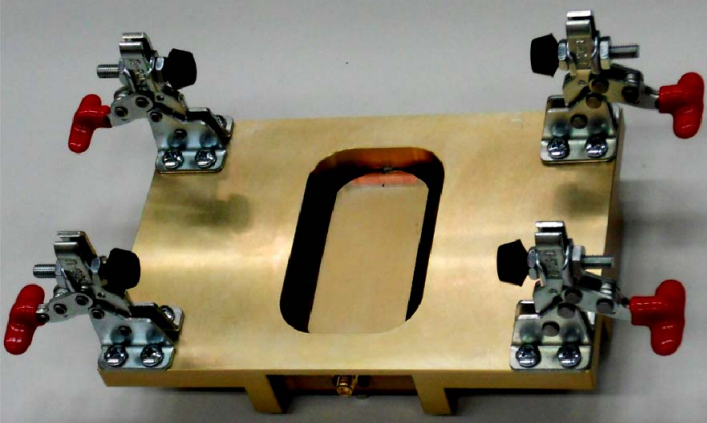
\includegraphics[width=0.6\textwidth]{src/1/figures/modified_tem_cell.png}
  \caption{Modified TEM cell from \cite{SDRAMCase}}
  \label{fig:modified-tem-cell}
\end{figure}

B. Orr reports in \cite{softFailSubsystem} errors caused by electrostatic discharges on two different camera communication buses.
Events of different severities are observed, depending on the discharge parameters.
It is attempted to determine whether the sensor or the application processor is causing the error.
The magnetic emission map is recorded with a near-field magnetic scanner to try to observe local variations in the emission spectrum because of the degradation of functionnality.
It was envisionned that soft-failure can induce significant variations in the emission spectrum of a disturbed component, and thus those variations could help localize them.
In this particular case, the root cause of failures could not be determined.

An LCD display is studied in \cite{softFailLCD}.
The device is tested with an IEC 61000-4-2 \cite{iec61000-4-2} generator, and non-destrutive problems are observed due to the discharge.
Electromagnetic disturbances cause stripes to appear on the display, optical parameters changes and blacklighting malfunctions.
System-level testing waveforms were found too complex for identifying the root cause.
A near-field injection is performed to identify which trace of the LCD's flex connector claims the lowest immunity.
The lack of resolution of the near-field probe caused multiple traces to be disturbed at once, preventing this second approach to work.
Finally, the individual track stressing was repeated with a capacitively-coupled \gls{tlp} on each individual metal track.
However, results were once more unconclusive and no metal trace could categorically be identified as more sensitive than the others.
The conclusion for this paper is that silicon level soft-error models are required for standard investigation.

An investigation method is presented in \cite{softFailMobile} to search for discharge propagation paths responsible for soft-failures on a mobile phone.
The IEC 61000-4-2 standard is chosen as testing waveform.
Metallic parts are assumed to be the main propagation paths.
To confirm this hypothesis, time-domain electromagnetic field 3D simulations of almost the entire phone are ran (see Fig. \ref{fig:mobile-phone-3d-em})
After the failure location was determined, RC-networks are used as countermeasures to protect physical inputs and outputs, like buttons, LCD inputs and connectors.

\begin{figure}[!h]
  \centering
  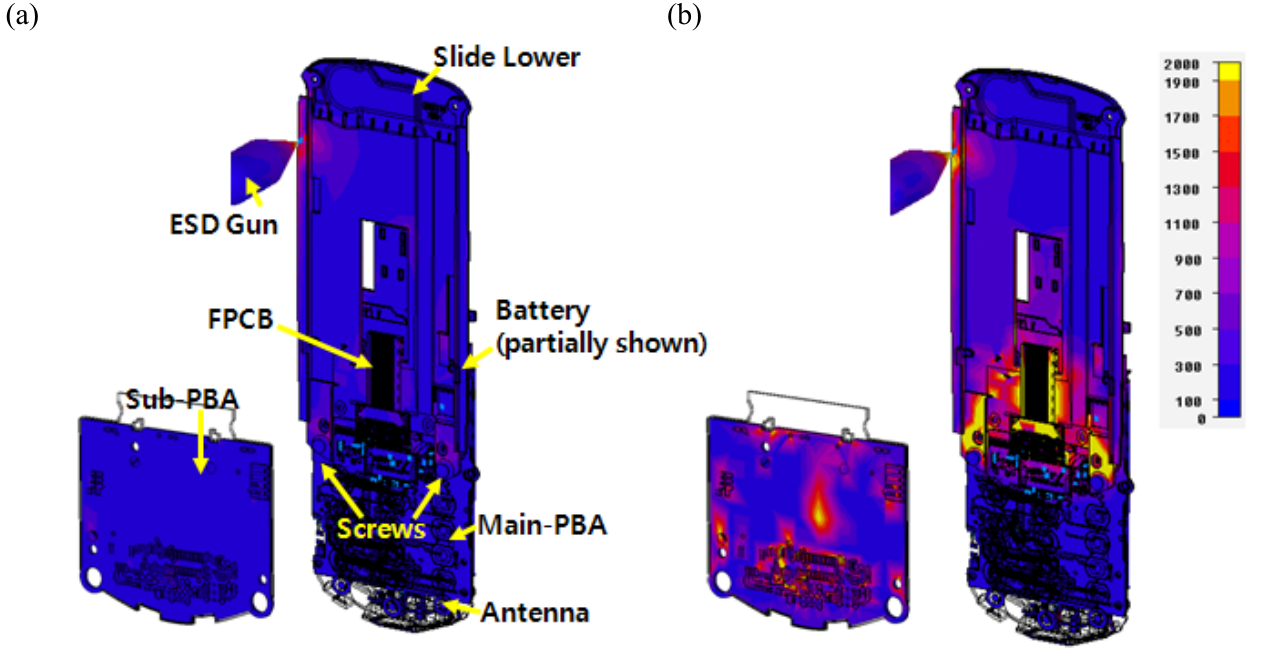
\includegraphics[width=0.8\textwidth]{src/1/figures/current_distribution_mobile.png}
  \caption{ESD Current Distribution on Mobile Phone and Backside sub-battery pack at (a) 1.0 ns and (b) 1.8 ns (Credit: \cite{softFailMobile})}
  \label{fig:mobile-phone-3d-em}
\end{figure}


Near-field scan

% Introduce near-field scanner
Electromagnetic near-field scanner measure maps of electric and magnetic field.
An electric or magnetic probe is swept closely above a device to record the emitted field in near-field conditions.
Measurements may be carried out in the frequency domain or in the time domain.
This tool was initially intended for architectural analysis such as floor-planning and power distribution analysis.
For ESD, spatial information provided by the recorded map is very useful to locate failures and malfunctions.
A comprehensive and detailed analysis of near-field antennas is done by A.D. Yaghjian in \cite{nfsFirstStudy}.
More recent work details the principle of operation, data processing and hardware requirements in \cite{near-field-scan, planarNFSAntenna, NFSMeasurements, NFScanner}.
Finally, measurement of electromagnetic emissions with surface scan method is standardized in IEC TS 61967-3 \cite{iec61967}.
The architecture of a near-field scanner is given in Fig. \ref{fig:near-field-scanner}.

\begin{figure}[!h]
  \centering
  \includegraphics[width=0.4\textwidth]{src/1/figures/architecture_near_field_scanner.pdf}
  \caption{Architecture of a near-field scanning testbench}
  \label{fig:near-field-scanner}
\end{figure}

\begin{figure}[!h]
  \centering
  \includegraphics[width=0.4\textwidth]{src/1/figures/near_field_scanner_susceptibility_map.pdf}
  \caption{Susceptibility map of a board recorded with surface scan in injection configuration \cite{}}
  \label{fig:near-field-scan-map}
\end{figure}

Revue des méthodes de modélisation

In the litterature, various ESD modelling methods can be found.
They comprise a wide range of techniques such as 3D electromagnetic and semiconductor physics simulations, compact, behavioral, physically-based and non-linear modelling.
The methods described hereafter could be used for soft-failure investigation.

M. Scholz details a mixed-mode ESD simulation approach in \cite{mixedModeESDSims}.
It is a combination of \gls{spice} and \gls{tcad} models, simulated in \gls{spice} environment.
The author indicates that the combination of physical device models and standard simulations provides higher accuracy and more realistic simulations than behavioral \gls{spice} models.
Using this complex simulation tool, on-chip and off-chip device interactions are studied, in powered and unpowered conditions.

In \cite{usb2ESDProtection}, TLP characterizations serves as an I(V) model for both external protections and an \gls{ic} pin.
The \gls{pcb} S-parameters are extracted from the board layout, using Momentum software (Agilent Technology).
It is electrically model with lumped R,L,C,G elements.
The modelling approach proved successful for simulation interactions between external devices and on-chip structures.
This method is interesting for soft-failure analysis because it is thorough and complete and enables accurate ESD simulation.

% IBIS is not enough for modelling an IC pin for ESD simulations
The Input Output Buffer Information Specification (IBIS) \cite{ibis-spec} is a behavioral, black-box model for performing signal integrity simulation on digital circuits.
It is widespread in the digital \gls{asic} world because it enables accurate simulations without disclosing circuit or process information.
It was envisionned that IBIS models could also be used or extended for ESD.
It is demonstrated in \cite{ibisImprovementFabrice} that the model lacks some parameters for EMC and ESD simulations.
It comprises a current versus voltage characteristic of \gls{io}s, similar to what can be extracted by a TLP, however the IBIS model is not defined for fast impulses and high injection.

N. Lacrampe proposes in \cite{LacrampeTransientImmunity} to perform 3D electromagnetic simulations at silicon level, using the integrated circuit layout, to deduce the amount of capacitive couplings between Vdd and Vss rails.
The extraction is performed with HFSS software (Ansoft).
The goal of this analysis is to predict the susceptibility of integrated circuits against electrostatic discharges.
\gls{pcb} tracks are modeled by a distributed RLC network.
The package data from the IBIS model \cite{ibis-spec} was used in the simulations.
Finally, a TLP stress generator is modelled using a lookup table I(V) component, in series with a 50\textOmega{} resistor.

Once again, electromagnetic fullwave simulations are conducted in powered-on ESD analysis in \cite{softFailMobile}.
System-level components are simulated, such as PCB, metallic casing and battery back.
3D EM simulations helps to identify the main discharge paths and locate the failure.

\chapter{Développement d'outils logiciel et matériel d'investigation}
\label{chap:2}
\section{Méthode de modélisation au niveau système}

% Need to simulate from source to input for soft-failure analysis
Un environnement de test ESD est composé d'éléments récurrents tels que des sources DC, des oscilloscopes, des générateurs de stress et des cartes électroniques interconnectés par des câbles et des fils.
Les cartes électroniques embarquent différents types de composants, tels que des composants passifs, des protections ESD et des circuits intégrés.
Afin de simuler le comportement de tous ces éléments pendant une décharge ESD, une méthodologie de modélisation au niveau système est proposée.
Elle permet une simulation précise jusqu'à l'entrée d'un circuit intégré en fonctionnement.
L'objectif de la méthode proposée est tout d'abord de construire une librairie des éléments les plus courants, puis d'assembler ces éléments ensembles pour former le modèle complet du système à étudier.

% Cables and delays identified as important for esd sims - because of similar order of magnitude
Les câbles sont des éléments importants mais parfois négligés dans les simulations ESD.
Ils introduisent des délais de propagation non négligeables par rapport à la durée d'un ESD.
Pour ordre de grandeur, un câble coaxial 50\textOmega{} possède une constante de propagation d'environ 5 ns/m.
En comparaison, un ESD dure entre une dizaine et plusieurs centaines de nanosecondes, ce qui est globalement proche du même ordre de grandeur.
Les câbles sont avant tout des lignes de transmission, dont l'analyse théorique fut faite par J. Maxwell, L. Kelvin et O. Heaviside et énormément étudiées par la suite dans la littérature \cite{branin-tl-ref, hf-coax,lossy-tl,emc-analysis-tl}.

% Distributed model
Le modèle le plus populaire de ligne est basé sur des éléments distribués.
Concrètement, c'est une suite réseaux L-C tels que la Fig. \ref{fig:dis-line-model}.
Les valeurs de chaque élément sont calculées à partir des propriétés du câble et de la précision requise pour la simulation.

\begin{figure}[!h]
  \centering
  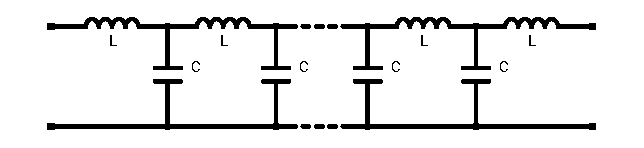
\includegraphics[width=0.7\textwidth]{src/1/figures/lc_ladder.pdf}
  \caption{Modèle de ligne de transmission LC distribué}
  \label{fig:dis-line-model}
\end{figure}

% Perks and disavantages
Malgré sa très large adoption, ce modèle présente de sérieux inconvénients.
En particulier, ce modèle nécessite un très grand nombre d'éléments pour avoir une précision correcte de simulation de câbles longs tels que le câble de 10m d'un TLP.
Pour une même précision, le nombre d'éléments est proportionnel à la longueur du câble, ce qui augmente considérablement les temps de simulation.
Pour augmenter la bande passante du modèle, le nombre d'éléments doit également être augmenté.
La combinaison des deux résulte en des temps de simulation très longs.

% Behavioral model
Le modèle à deux ports décrit par H. Branin \cite{branin-tl-ref} est une alternative bien plus performante au modèle distribué.
Il décrit très efficacement et avec une très grande précision le comportement d'une ligne de transmission.
La bande passante n'est pas limité, et le temps de simulation est indépendant de la longueur du câble.
Le modèle est constitué de deux sources de tension contrôlées en tension et deux résistances (Fig. \ref{fig:beh-line-model}).

\begin{figure}[!h]
  \centering
  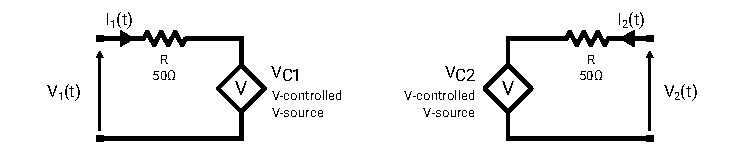
\includegraphics[width=\textwidth]{src/1/figures/behavioral_line_model.pdf}
  \caption{Modèle comportemental d'une ligne de transmission sans pertes}
  \label{fig:beh-line-model}
\end{figure}

Les équations définissant le comportement des sources de tension sont données dans le document final.
Elles décrivent un système où tension et courant à chaque port sont la superposition d'une onde se propageant dans un sens et d'une seconde dans l'autre sens.

% Model other devices
La modélisation d'autres éléments importants tels que les composants passifs et les protections ESD est détaillé dans le document complet.

% Illustrate the method with a practical case
Pour illustrer l'application de la méthode de modélisation, elle est appliquée sur un banc TLP du laboratoire de NXP Toulouse.
C'est un bon cas d'étude afin d'utiliser la méthode, car ce banc est très largement utilisé pour l'investigation.
Pour démontrer sa précision, le modèle est vérifié par comparaison avec de multiples mesures, sous différentes charges et amplitudes.

\begin{figure}[!h]
  \centering
  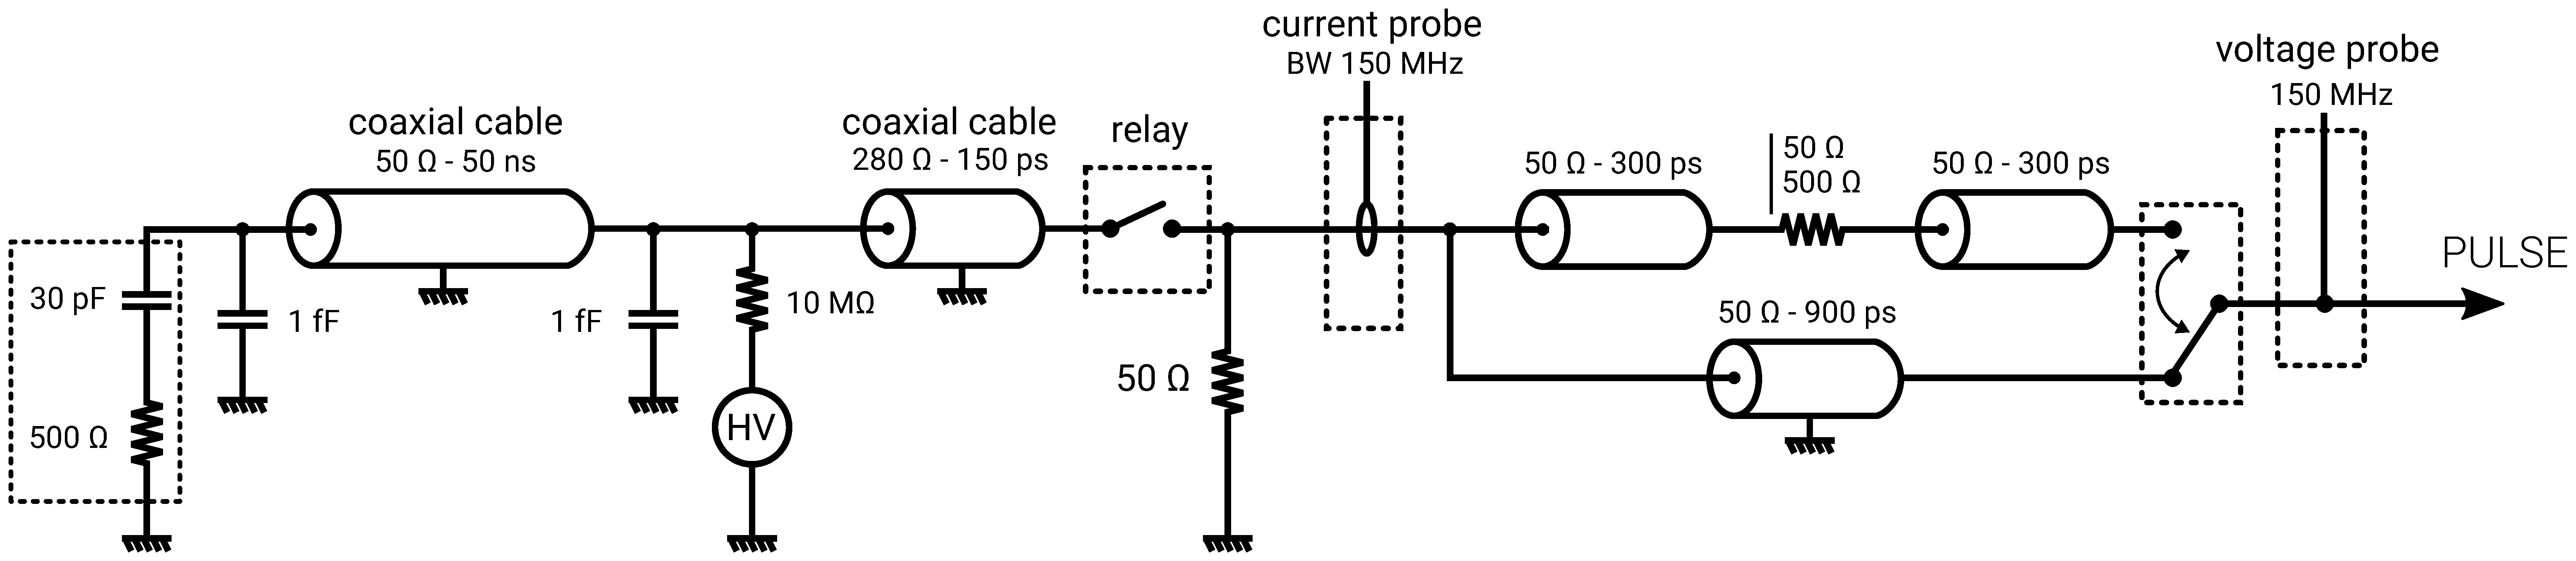
\includegraphics[width=\textwidth]{src/1/figures/complete_nxp_tlp_model.pdf}
  \caption{Modèle complet du générateur TLP du laboratoire NXP Toulouse}
  \label{fig:complete-tlp-model}
\end{figure}

% Explain how the model, how it was constructed
Le modèle complet de TLP est donné en Fig. \ref{fig:complete-tlp-model}.
Il reproduit l'architecture du TLP du laboratoire en utilisant des modèles de la librairie pour chaque élément.

% Detail a first comparison with 25 ohms
Une première comparaison entre une mesure et simulation est donnée en Fig. \ref{fig:comparison-tlp-load}.
Avec une charge de 25\textOmega{} et une tension de charge de 500 V, un courant de 4.5 A et une tension de 125 mV sont relevés sur le second plateau de la courbe.
Le rapport de ces deux valeurs corresponds bien à 25\textOmega{} comme attendu.
Jusqu'à 220 ns, les deux courbes se ressemblent fortement.
Après 220ns, des différences apparaissent, supposées dues aux erreurs de modélisations.
La plupart des simulations ESD restent intéressantes pendant la partie principale de la décharge jusqu'à 120 ns et ces erreurs sont donc négligeables.

\begin{figure}[!h]
  \centering
  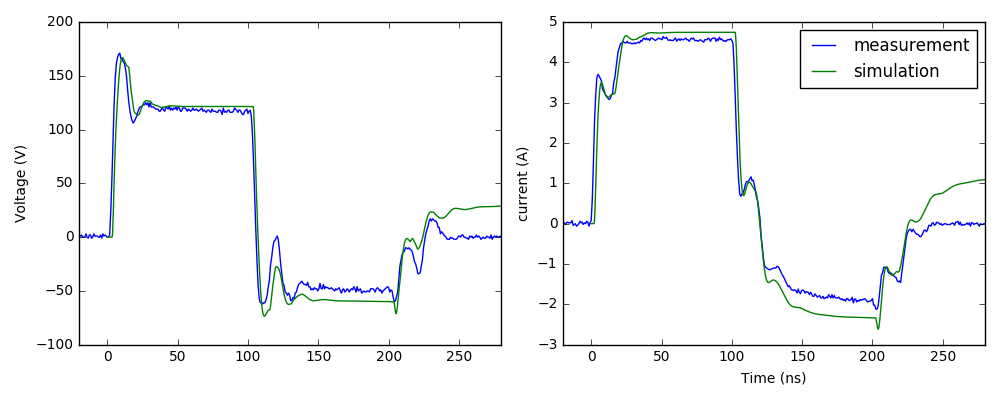
\includegraphics[width=\textwidth]{src/1/figures/tlp_comparison_R25_500V.png}
  \caption{Comparaison des courbes temporelles de tension et courant avec une  tension de charge 500 V sous 25\textOmega{}}
  \label{fig:comparison-tlp-load}
\end{figure}

% More validations in Annex
Les autres validations sont données dans le document complet, et présentent des niveaux de corrélations aussi proches.
Le modèle fonctionne correctement et reproduit les mesures, prouvant sa validité.

\section{Développement d'un générateur TLP modifié}

% TLP is a great tool for esd analysis
Le TLP est capable de générer des impulsions très bien contrôlées et reproductibles.
L'utilisation des pistolets ESD reste obligatoire pour la qualification de produits.
La forme d'onde la plus répandue est celle définie dans la spécification HMM \cite{hmm} et les standards IEC 61000-4-2 \cite{iec61000-4-2} et ISO 10605 standard \cite{iso10605}.
Ensemble, ils couvrent une très large plage d'applications, dans les domaines grand-public, automobile et industriel.
Pour combiner les avantages d'un TLP avec ceux d'une décharge HMM, un générateur TLP peut être modifié pour produire cette impulsion HMM.
Cette approche a été explorée par le passé par E. Grund \cite{iec61000-tlp} et Y. Cao \cite{tlp-based-hmm}.
Néanmoins, leurs techniques présentent quelques inconvénients tels que une tendance large à créer des oscillations, comme démontré dans le document complet.

Le générateur proposé ici est dénommé TLP-HMM.
Le TLP-HMM requiert deux modules additionnels à connecter à chaque extrémité d'un TLP standard 100 ns.
Ils sont nommés \textit{absorber} et \textit{shaping filter} (Fig. \ref{fig:tlp_hmm_architecture}).
Le principe du TLP-HMM est de re-router une portion du courant incident dans la masse, de manière à ce que le courant restant prenne la forme de l'onde HMM.
Le fonctionnement de chaque élément est détaillé dans le document final.

\begin{figure}[!h]
  \centering
  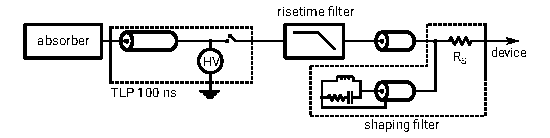
\includegraphics[width=0.9\textwidth]{src/1/figures/beges_tlp_hmm.pdf}
  \caption{architecture du TLP-HMM}
  \label{fig:tlp_hmm_architecture}
\end{figure}

Les courbes simulées et mesurées sur un prototype sont données Fig. \ref{fig:tlp_hmm_waveforms}.
Les courants mesurés à 30 ns et 60 ns sont dans la marge de tolérance de 30\% des standards, et elle est donc valide.

\begin{figure}[!h]
  \centering
  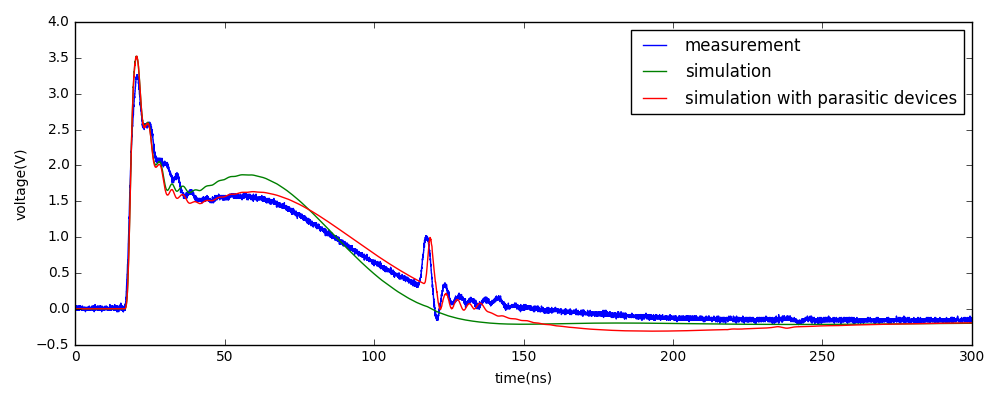
\includegraphics[width=0.95\textwidth]{src/1/figures/tlp_hmm_waveforms.png}
  \caption{Mesure et simulation d'une décharge 250 V TLP-HMM (équivalente 1 kV HMM) sur 2\textOmega{}}
  \label{fig:tlp_hmm_waveforms}
\end{figure}

% Analyse the curve
Globalement, la simulation et la mesure corrèlent bien.
Il y a des différences mineures, notamment entre 40 ns et 150 ns.
Elles sont dues à des éléments parasites non pris en compte durant les simulations, et des corrections sont à apporter au prototype.
L'analyse de ces éléments est fournie dans le document complet.

\section{Méthode de traitement de capteurs de courant on-chip}

% Introduction
Avec une mesure de champ-proche, il est possible de mesurer des cartographies de champ électrique ou magnétique.
Dans ce chapitre deux méthode de reconstruction sont évaluées afin de retrouver des valeurs de courant depuis une cartographie de champ magnétique.
Le capteur de champ proche sur silicium présenté dans le chapitre 4 est utilisé pour obtenir des mesures de courant sur puce.

% What is the output voltage that is measured
La méthode temporelle consiste simplement à intégrer le signal mesuré en y appliquant des facteurs correctifs.
Il est montré dans \cite{near-field-scan} que cette approche est valide.
Le schéma de la méthode de mesure est donnée Fig. \ref{fig:calibration-sensor}.
Une impulsion rectangulaire de 100 ns et 1 V est injectée entre S1 et S2.
La tension V\textsubscript{sensor} est mesurée avec un oscilloscope 2 GHz entre C1 et C2.

\begin{figure}[!h]
  \centering
  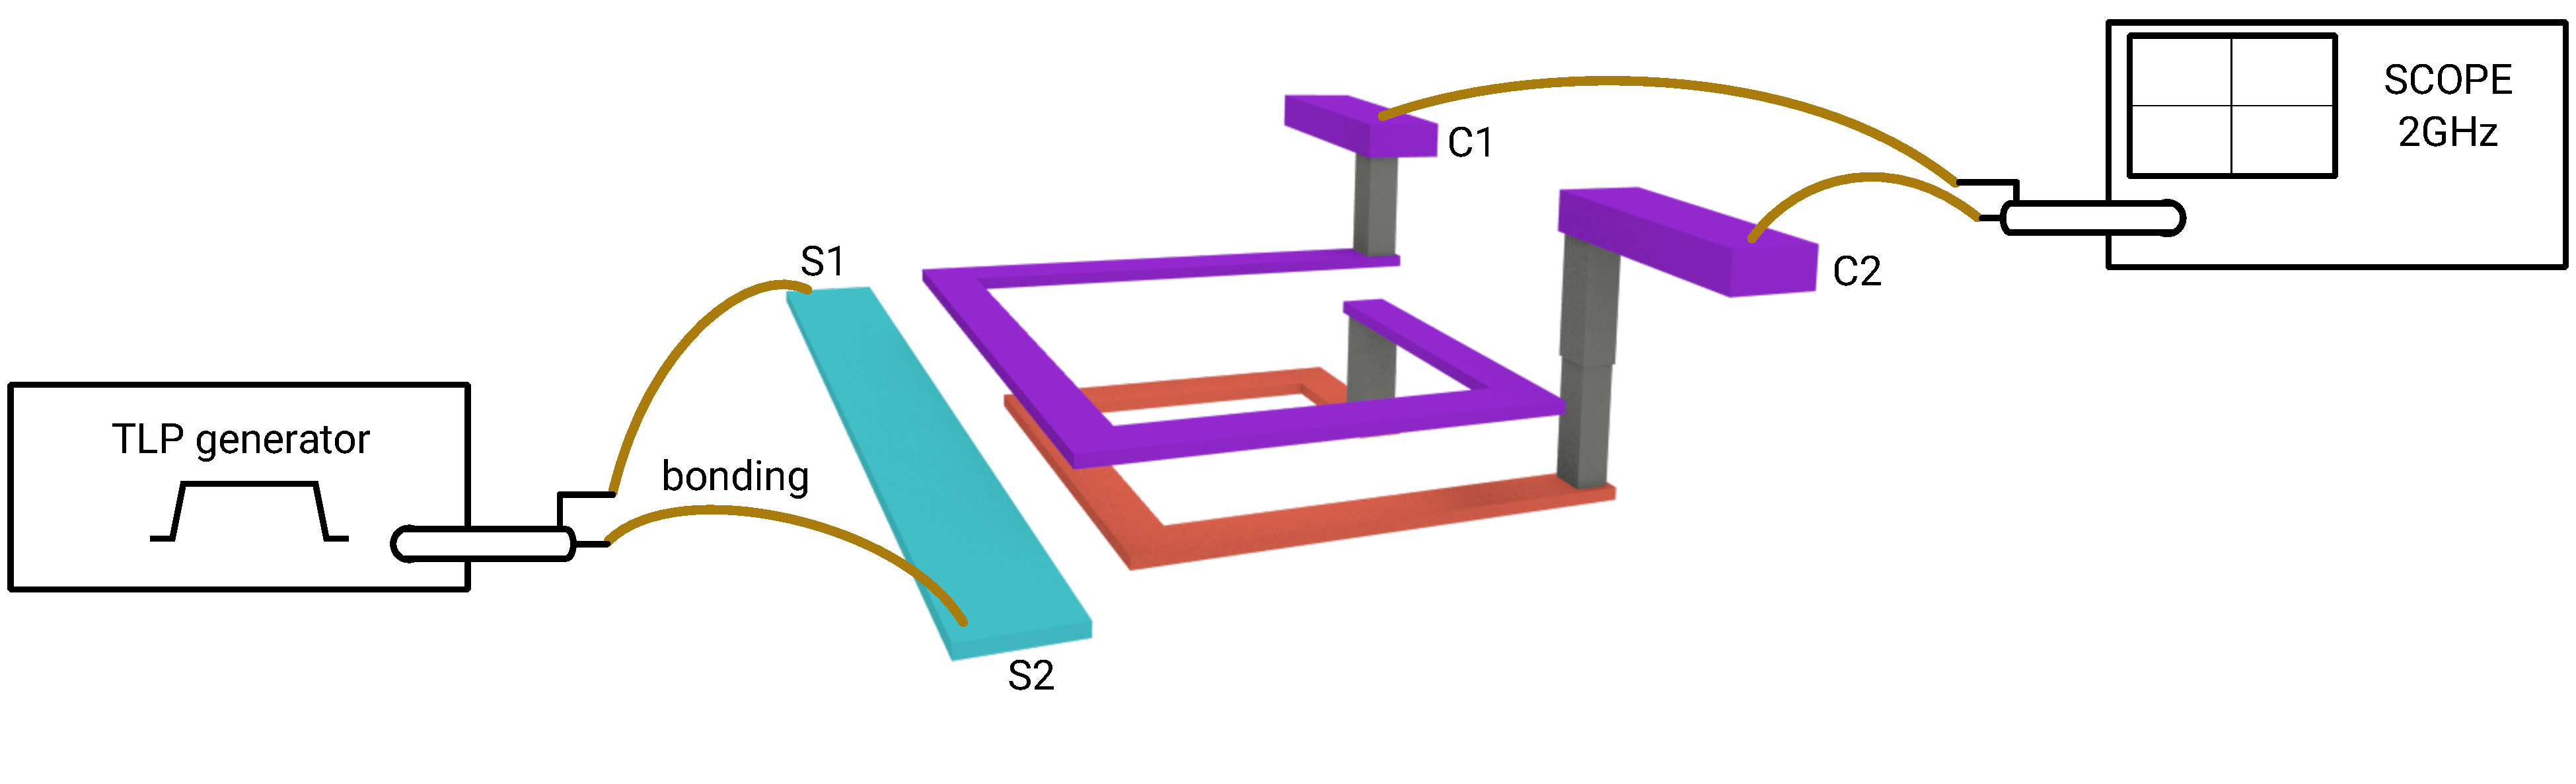
\includegraphics[width=0.9\textwidth]{src/1/figures/sensor_measurement_setup.pdf}
  \caption{Montage de calibration du capteur de courant sur silicium dans le domaine temporel}
  \label{fig:calibration-sensor}
\end{figure}

% Intro & Characterization
La méthode fréquentielle utilise une mesure paramètre-S du capteur pour traiter V\textsubscript{sensor}.
Le montage de calibration est similaire à la méthode temporelle et donnée dans le document final.
Elle est basée sur une utilisation de la réponse fréquentielle du capteur pour corriger les mesures temporelles.

Une comparaison de la courbe originale, de la méthode temporelle, et de la méthode fréquentielle sont fournies Fig. \ref{fig:freq-domain-reconstructed}.
Globalement, les résultats sont similaires en terme de précision.
La courbe mesurée est obtenue par reflectométrie, ce qui explique pourquoi elle possède plusieurs plateaux contrairement aux simulations.
De multiples améliorations sont possibles pour les deux méthodes, et des pistes sont proposées dans le document final.

\begin{figure}[!h]
  \centering
  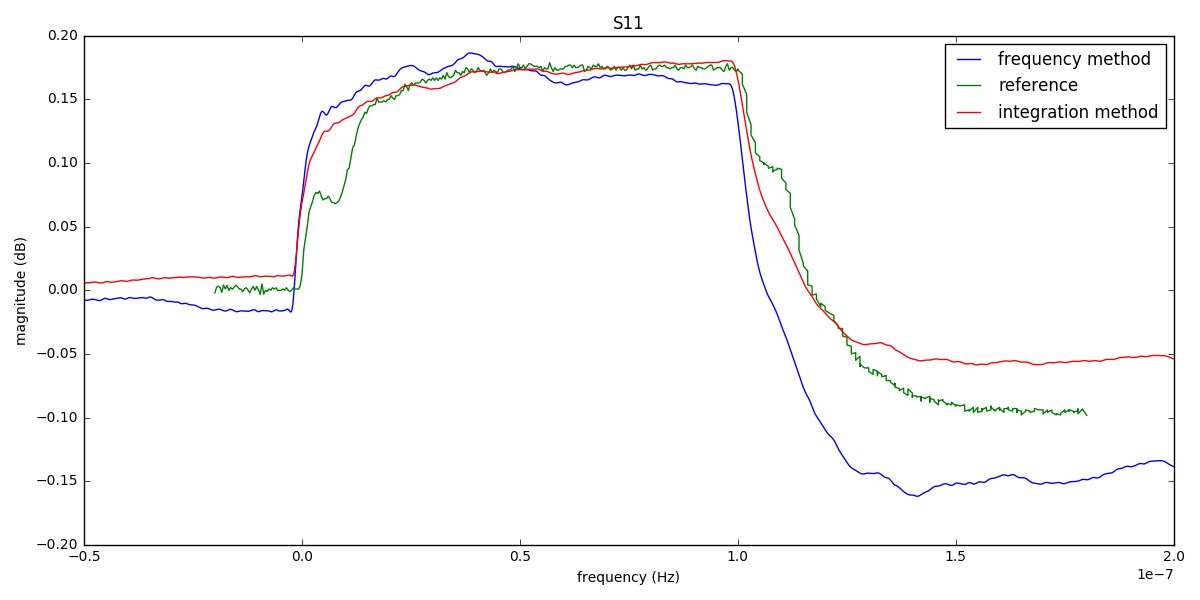
\includegraphics[width=0.9\textwidth]{src/1/figures/final_comparison_reconstructions.png}
  \caption{Courant de référence, reconstruction par méthode temporelle et fréquentielle}
  \label{fig:freq-domain-reconstructed}
\end{figure}

\chapter{Étude de cas - défaillance circuit intégré}
\label{chap:3}
\section{Présentation du produit et de la défaillance}

Ce travail de recherche a pour but d'étudier et de prédire les pertes de fonctionnalités causées par des décharges électrostatiques.
Dans ce chapitre, un cas réel de défaillance fonctionnelle est présenté.
Il a été identifié sur un circuit intégré automobile spécifique, qui a pour responsabilité des tâches critiques et de haut-niveau dans le véhicule.
Cette défaillance a été détectée en réduisant la quantité de composants externes au niveau de la carte, dans le but de diminuer la BOM (Bill Of Materials) et donc le coût de l'application complète.
Dans la campagne de tests, les décharges sont injectées à travers la connexion batterie (Fig. \ref{fig:system_architecture}).

\begin{figure}[!h]
  \centering
  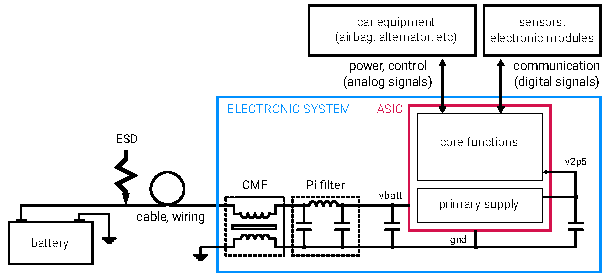
\includegraphics[width=0.9\textwidth]{src/1/figures/architecture_system.pdf}
  \caption{Vue d'ensemble de l'architecture du système}
  \label{fig:system_architecture}
\end{figure}

% Main task
La tâche en défaillance est une fonction de régulation, chargée principalement de convertir la tension batterie en une alimentation régulée 2.5 V.
Plusieurs sous-fonctions (aussi appelées blocs) traitent la tension batterie dans ce but.
L'architecture de la fonction intégrée est donnée Fig. \ref{fig:monitored_function}).

\begin{figure}[!h]
  \centering
  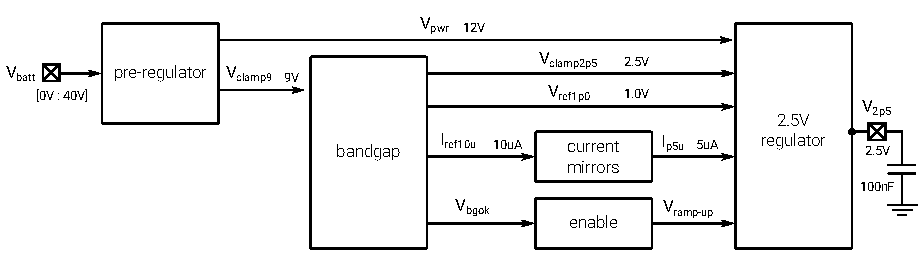
\includegraphics[width=0.9\textwidth]{src/1/figures/monitored_function.pdf}
  \caption{Architecture du primaire d'alimentation}
  \label{fig:monitored_function}
\end{figure}

% First block
Le pré-régulateur limite la tension d'entrée V\textsubscript{batt} pouvant atteindre jusqu'à 40 V, et fournit le signal V\textsubscript{clamp9}.
V\textsubscript{clamp9} alimente les blocs internes à faible consommation, tandis que V\textsubscript{pwr} fournit un plus large courant sous 12 V.
% Second block
Ensuite, une référence bandgap génère, après un délai de démarrage, notamment une référence à 1.0 V appelée V\textsubscript{ref1p0}.
Le bandgap fournit aussi une référence de courant à 10\textMu{}A sur I\textsubscript{ref10u}, ainsi qu'un drapeau V\textsubscript{bgok} pour signaler si il est en fonctionnement nominal ou non .
% Third major block
Enfin, le régulateur faible-pertes génère une alimentation stabilisée 2.5 V sur V\textsubscript{2p5}, avec une capacité en courant jusqu'à 20 mA.
V\textsubscript{2p5} sert ensuite à alimenter des cellules digitales à l'intérieur du circuit intégré.

% Principe défaillance
La défaillance de ce système est observée sur V\textsubscript{2p5} (Fig. \ref{fig:meas-reset-v2p5}).
Elle est induite en injectant une forte impulsion transitoire d'amplitude négative sur V\textsubscript{batt}, lorsque le produit est alimenté et en fonctionnement normal.
La durée de la défaillance sur V\textsubscript{2p5} (30 \textmu{}s) est bien plus longue que la perturbation d'entrée sur V\textsubscript{batt} (100 ns), ce qui semble indiquer une large faute fonctionnelle dans le circuit.

\begin{figure}[!h]
  \centering
  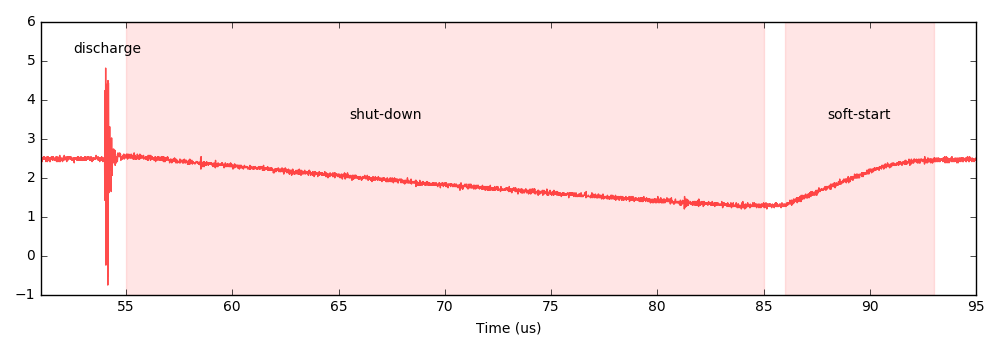
\includegraphics[width=0.9\textwidth]{src/1/figures/v2p5_measure.png}
  \caption{Mesure de V\textsubscript{2p5} après une stress rectangulaire -450 V 100 ns}
  \label{fig:meas-reset-v2p5}
\end{figure}

% What is the root cause -> reset of regulator, soft-start
Plus précisément, le stress négatif semble déclencher une séquence de démarrage, alors que le régulateur est normalement déjà démarré.
Pendant cette séquence, la tension d'alimentation monte doucement depuis 0 V jusqu'à 2.5 V, afin d'éviter des surtensions.
Ces séquences de démarrage sont logiquement longues et demandent un certain temps pour se terminer.
Si un ESD déclenche une telle séquence, le système se retrouve indisponible pendant un délai important.

La prochaine partie du travail de recherche est focalisé sur le développement de méthodes de mesures directement sur silicium.
L'objectif est d'acquérir des données fiables directement au niveau circuit, ce qui est difficile à faire de manière externe, et afin de valider les simulations pour l'investigation.
Notamment, un véhicule de test a été développé.
Il contient différentes méthodes de mesure et d'observation.

\section{Présentation du véhicule de test}

% Architecture
L'architecture du véhicule de test est donnée Fig. \ref{architecture_testchip}.
Il contient deux instances de la même fonction de régulation.
La première instance est la fonction sous-test, exposée à des décharges électrostatiques pendant la campagne de tests et dont le comportement est surveillé afin de détecter les fautes.
La seconde instance alimente justement les systèmes de surveillance qui sont directement intégrés sur puce.

\begin{figure}[h]
  \centering
  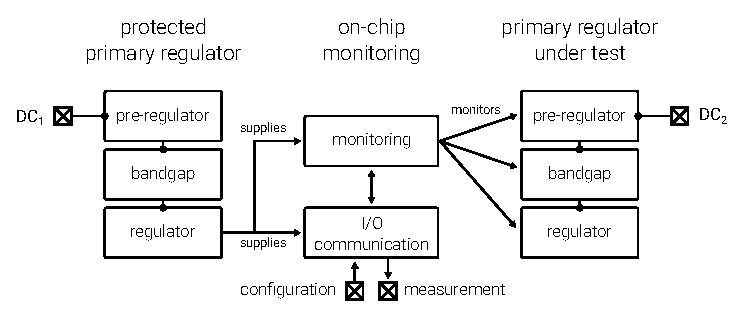
\includegraphics{src/1/figures/architecture_testchip.pdf}
  \caption{Architecture du véhicule de test}
  \label{architecture_testchip}
\end{figure}

Le layout top de la puce est donné Fig. \ref{fig:top-cell-layout}.
Il est possible d'identifier à droite et à gauche chaque instance de la fonction de régulation.
Les systèmes de surveillance sont localisés globalement de dessous de ces deux blocs.
Des capteurs de courant sur puce sont localisés à plusieurs endroit contre l'anneau de métal gndsub entourant toute la puce.
Beaucoup d'espace a été laissé libre sur le layout, pour des contraintes de fabrication.

\begin{figure}[!h]
  \centering
  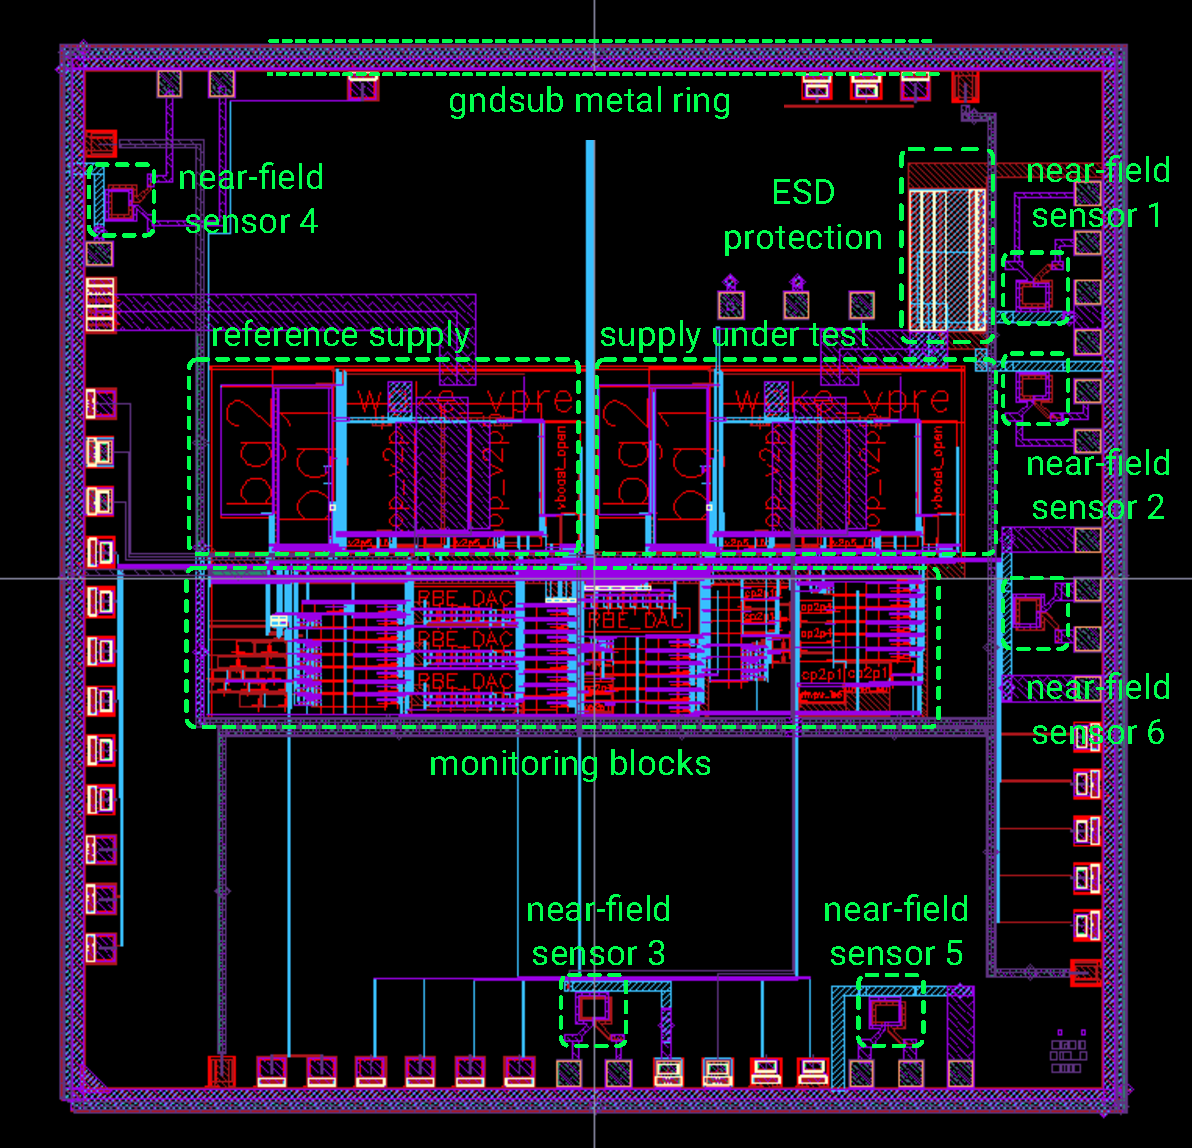
\includegraphics[width=0.7\textwidth]{src/1/figures/topcell_layout.pdf}
  \caption{Layout de la top-cell}
  \label{fig:top-cell-layout}
\end{figure}

% What is in the monitoring system
Les systèmes de surveillance contiennent notamment des détecteurs de surtension et sous-tension.
Il y a au total 35 détecteurs de ce type dans la puce.
Ils sont implémentés avec des comparateurs verrouillés
Un drapeau est levé si un nœud surveillé dépasse un niveau de référence.
Une fois le drapeau levé, il est maintenu jusqu'à ce que la cellule puisse être lue et remise � z�ro.
L'architecture est donnée Fig. \ref{fig:architecture-ov}.

\begin{figure}[!h]
  \centering
  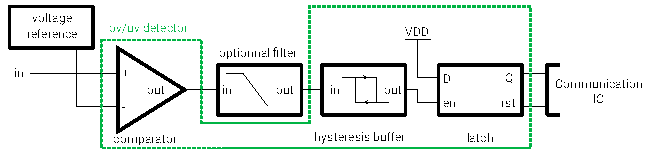
\includegraphics[width=0.9\textwidth]{src/1/figures/architecture_OV.pdf}
  \caption{Architecture du détecteur de surtension}
  \label{fig:architecture-ov}
\end{figure}

% Detail architecture
Dans cette architecture, la comparaison est réalisée par le comparateur, implémenté avec un amplificateur opérationnel à deux étages avec un buffer de sortie.
Cette topologie convient bien pour des comparateurs à fort gain, travaillant en boucle ouverte avec une très forte impédance d'entrée, afin de ne pas perturber le circuit.
A la sortie du comparateur, un filtre RC optionnel peut être connecté.
Il permet d'éliminer les surtensions les plus courtes afin de détecter seulement de larges perturbations.
Ensuite, un buffer à hystérésis permet de maximiser l'efficacité du filtre et d'obtenir une valeur numérique robuste de la sortie du comparateur.
Finalement, une bascule D garde le drapeau en mémoire une fois levé.
Si le buffer à hystérésis devient haut, la bascule recopie un état haut sur sa sortie.

% Origin of reference voltages
Les tensions de références de ces détecteurs sont soit fixes, soit contrôlables via un bus de communication.
Par ailleurs, tout ces détecteurs peuvent être lus par un second bus de communication.
Ce bus fonctionne sur le principe d'une chaine JTAG.
Des cellules individuelles peuvent être connectées en chaine afin de former un bus de la longueur désiré.
Cette approche est très pratique pour monter rapidement un véhicule de test.
Néanmoins, des problèmes important furent rencontrés avec ces bus de communication.
Ils sont exposés en détail dans le document complet.

% What is a current sensors
Dans le véhicule de test, on trouve également des capteurs de courant directement intégrés sur silicium.
Chaque capteur est placé à proximité de la piste de métal à mesurer.
Par couplage, il génère une tension proportionnelle à la dérivée du courant dans la piste.

Les figures \ref{fig:near-field-current-sensor} et \ref{fig:near-field-current-sensor-layout} fournissent respectivement une représentation 3D du capteur ainsi que son layout.
Ce type de boucle de courant intégré sur silicium a été originellement désigné et étudié par A. Salles dans \cite{AlainSallesInductors}.

\begin{figure}[!h]
  \centering
  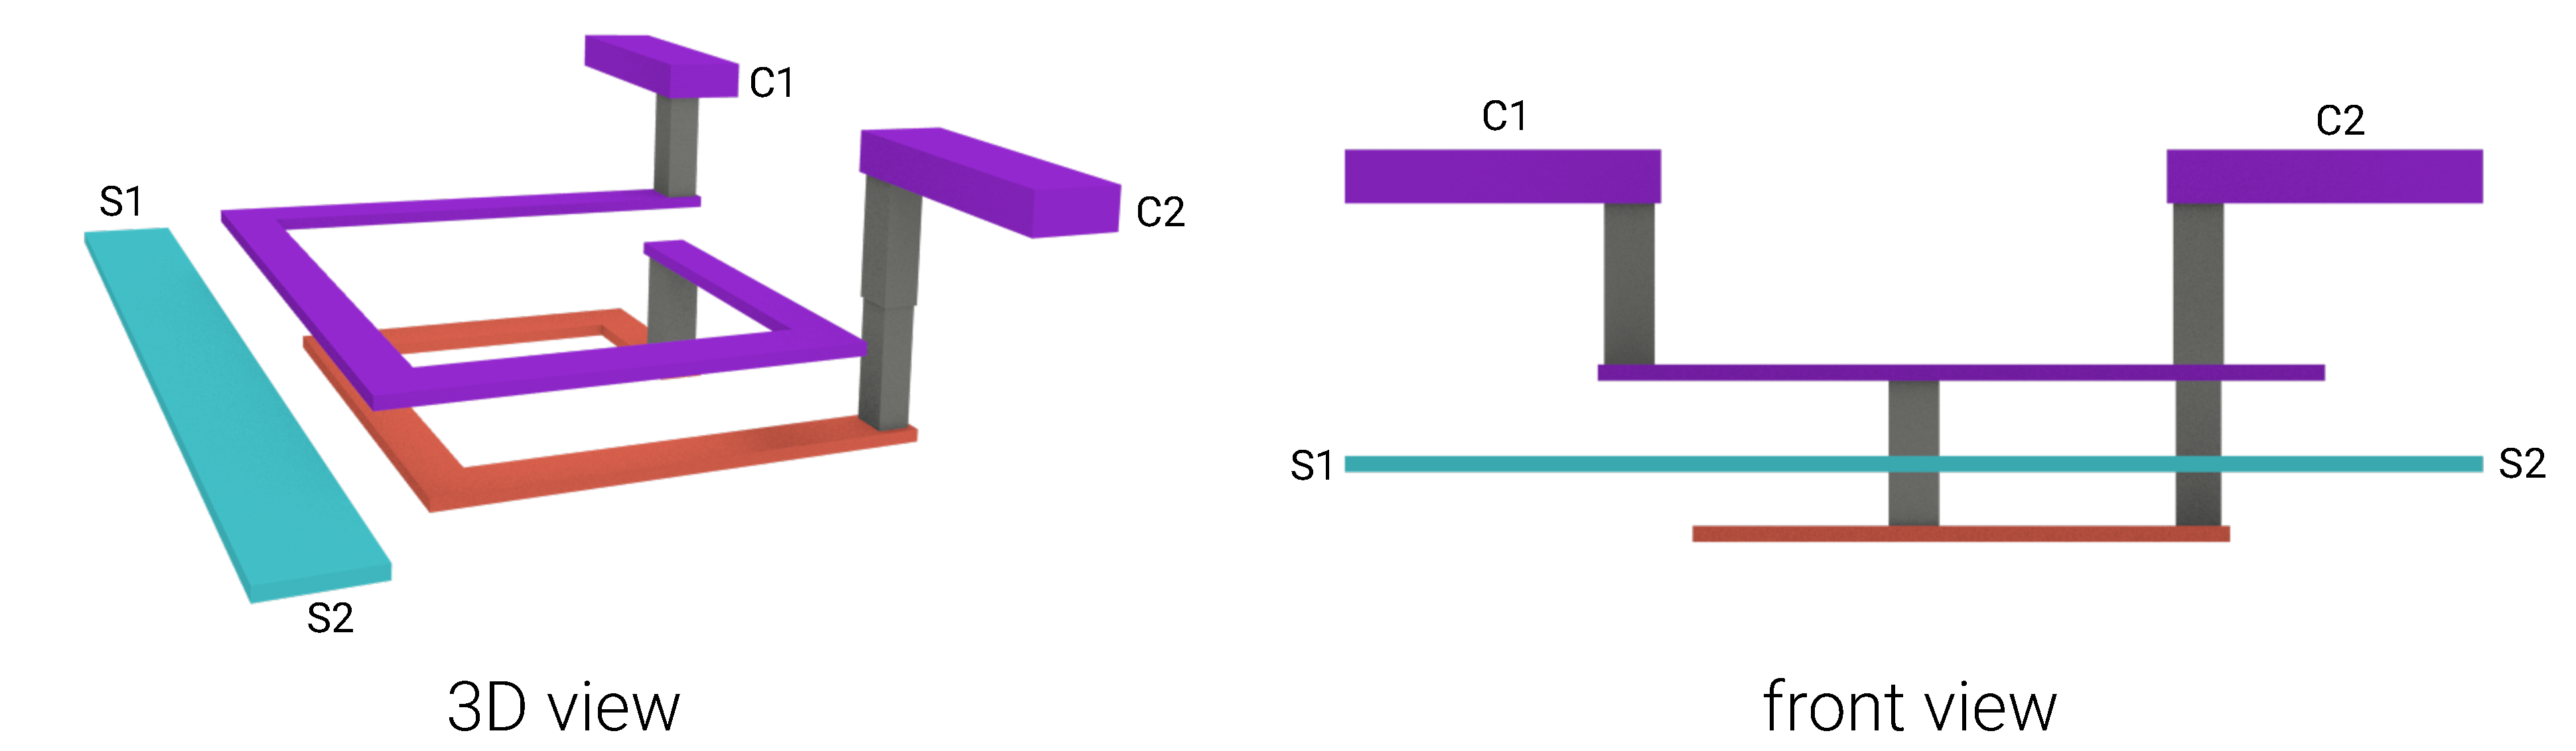
\includegraphics[width=0.98\textwidth]{src/1/figures/near-field-current-sensor.pdf}
  \caption{Design du capteur de champ-proche}
  \label{fig:near-field-current-sensor}
\end{figure}

% How is it designed and how is it used
Sur silicium, trois niveaux de métaux sont requis pour construire ce capteur.
Le premier niveau en rouge (Fig \ref{fig:near-field-current-sensor}) et le troisième niveau en violet forment une boucle métallique.
Des vias connectent les différents niveaux ensembles.
La piste mesurée est elle localisée au deuxième niveau.
Le courant mesuré circule entre les nœuds \textit{S1} et \textit{S2}.
Un oscilloscope avec une impédance d'entrée \textOmega{} est utilisé pour mesurer en différentiel la tension entre \textit{C1} et \textit{C2}.
Le traitement de la courbe obtenue a été détaillé précédemment dans le chapitre 2.

\begin{figure}[!h]
  \centering
  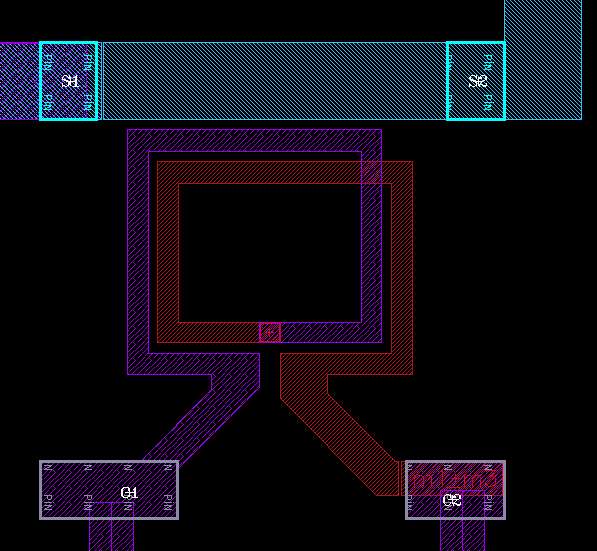
\includegraphics[width=0.5\textwidth]{src/1/figures/sensor_layout.png}
  \caption{Layout du capteur de champ proche}
  \label{fig:near-field-current-sensor-layout}
\end{figure}

% Talk about the near-field current sensors placement
Au total, il y a 6 capteurs de courant sur la puce.
Un des capteurs est dédié à la calibration, tandis que les autres mesurent des points d'entrée ou de sortie potentiels pour des ESD.
Le capteur \textit{1} mesure le courant sur l'entrée batterie.
Le capteur \textit{2} mesure le courant absorbé par la protection ESD protégeant l'entrée batterie.
Le capteur \textit{3} mesure le courant à travers la capacité externe de stabilisation du régulateur.
Enfin, les capteurs \textit{4} et \textit{5} mesurent les courants évacués via l'anneau métallique \textit{gndsub}, connecté extérieurement à la masse.

\chapter{Outils d'analyse de défauts fonctionnels ESD}
\label{chap:4}

Jusqu'à présent, l'étude s'est focalisée sur le développement de méthodes pour l'acquisition de données de mesures.
Ces mesures nécessitent la réalisation du circuit intégré afin de pouvoir le tester.
Ce procédé est couteux et intervient tard dans le flot de conception.
Les outils de simulation en revanche sont utilisables dés le début du flot de conception.
Ils peuvent donc largement compléter les systèmes de mesures présentés dans le chapitre précédent.
Dans ce chapitre-ci, deux méthodes différentes sont présentes.
La première est destinée aux concepteurs de circuits intégrés, tandis que la seconde vise plutôt les équipementiers.

\section{Méthode bottom-up}

% What is bottom up
L'approche présentée ici est apellée bottom-up, c'est à dire du bas vers le haut.
Elle consiste à caractériser de petites fonctions assez bas dans la hiérarchie du circuit intégré, de manière individuelle, puis d'assembler ensemble leurs modèles afin de déduire le comportement global.
Cett approche présente l'intérêt que des fonctions individuelles sont susceptibles d'être réutilisées, et donc que l'effort de charactérisation et de modélisation n'a besoin d'être fourni qu'une seule fois.
Un schéma de charactérisation assez simple est utilisé en simulation pour charactériser chaque bloc (Fig. \ref{block_function_cz}).
Il fournit l'alimentation nécessaire à la fonction qui doit être en fonctionnement.
Il permet également d'injecter sur une entrée un stress électrique et d'observer la réponse sur une sortie.

\begin{figure}[!h]
  \centering
  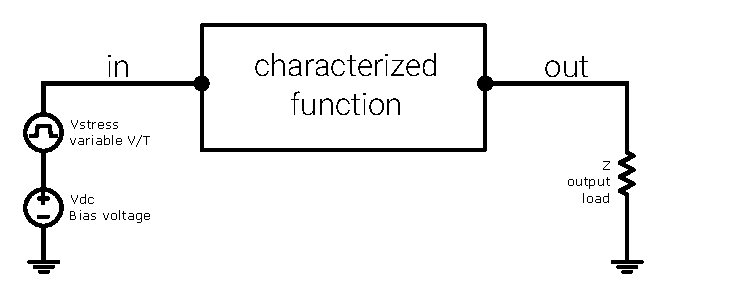
\includegraphics{src/1/figures/characterization_setup.pdf}
  \caption{Block characterization setup (supply input)}
  \label{block_function_cz}
\end{figure}

% What are the characterization signal
%TODO ref
Le signal de charactérisation est une impulsion rectangulaire, appliquée sur l'entrée sous test.
Un ensemble de simulations est effectué en faisant varier les paramètres de cette forme d'onde, injectée sur l'entrée.
Plus précisément, une analyse paramétrique est réalisée sur l'amplitude et la durée de l'impulsion.
Cet ensemble de simulations est résumé dans la Fig. \ref{set_input_signals}.
Cette méthode de charactérisation est fortement inspirée de la méthode Wunsch & Bell \cite{}.

%TODO: Fix sim 12 sim12
\begin{figure}[!h]
  \centering
  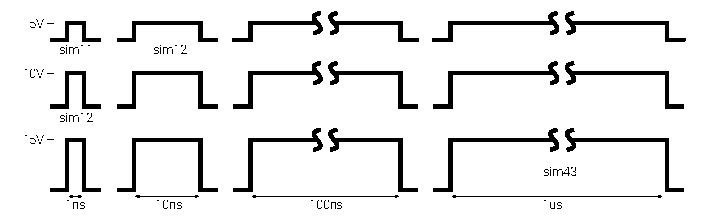
\includegraphics{src/1/figures/time_domain_cz_curves.pdf}
  \caption{Variations on (amplitude, duration) of the input characterization signal}
  \label{set_input_signals}
\end{figure}

Une fois chaque signal injecté, la sortie est observée.
Deux paramètres sont extraits de la forme d'onde de sortie.
L'amplitude maximale est extraite, correspondant à la plus large variation de tension par rapport à un niveau nominal.
La durée de cette variation, à 90\% de l'amplitude maximale est aussi relevée.
Ces deux paramètres permettent de décrire une boite englobante de la forme d'onde de sortie, constituant une sorte de forme d'onde simplifiée.
Cette analyse est effectuée pour chaque simulation.

Il en résulte deux tables, la première associant constituant le modèle du bloc.
La première table associes aux deux paramètres d'entrée (amplitude et durée) une amplitude maximale de sortie.
La seconde table associe aux deux paramètres d'entrée une durée de sortie.
Ces deux tables peuvent ensuite être intégrées dans un modèle, décrit Fig. \ref{fig:principle-transfert-func-v2}.
La fonction $F_{W}$ utilises la première table, pour retourner une amplitude de sortie en fonction des paramètres d'entrée.
La fonction $F_{V}$ utilises la seconde table et retourne une durée.
Sachant que ce modèle accepte les mêmes types de paramètres en entrée et en sortie, plusieurs modèles peuvent être chaînés les uns à la suite des autres, afin de reconstituer le comportement d'une fonction haut-niveau.

\begin{figure}[!h]
  \centering
  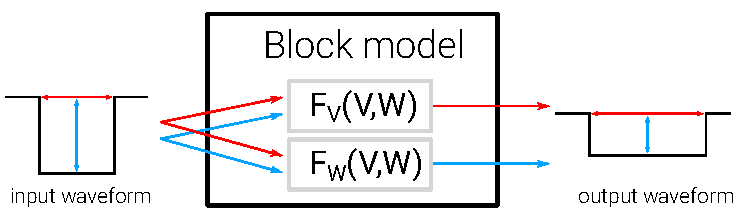
\includegraphics{src/1/figures/principle_transfert_function_v2.pdf}
  \caption{Improved modelling method}
  \label{fig:principle-transfert-func-v2}
\end{figure}

% First run the reference sim
Pour tester cette approche, des simulations sont effectuées en utilisant les schémas Fig. \ref{fig:hypothesis-setup}.
L'objectif est de comparer une simulation transistor de la fonction globale, à une chaine de simulation individuelle de blocs, pour vérifier si des réponses similaires peuvent être obtenues sur la broche de sortie lorsque la broche d'entrée est exposée au même stimuli.

\begin{figure}[!h]
  \centering
  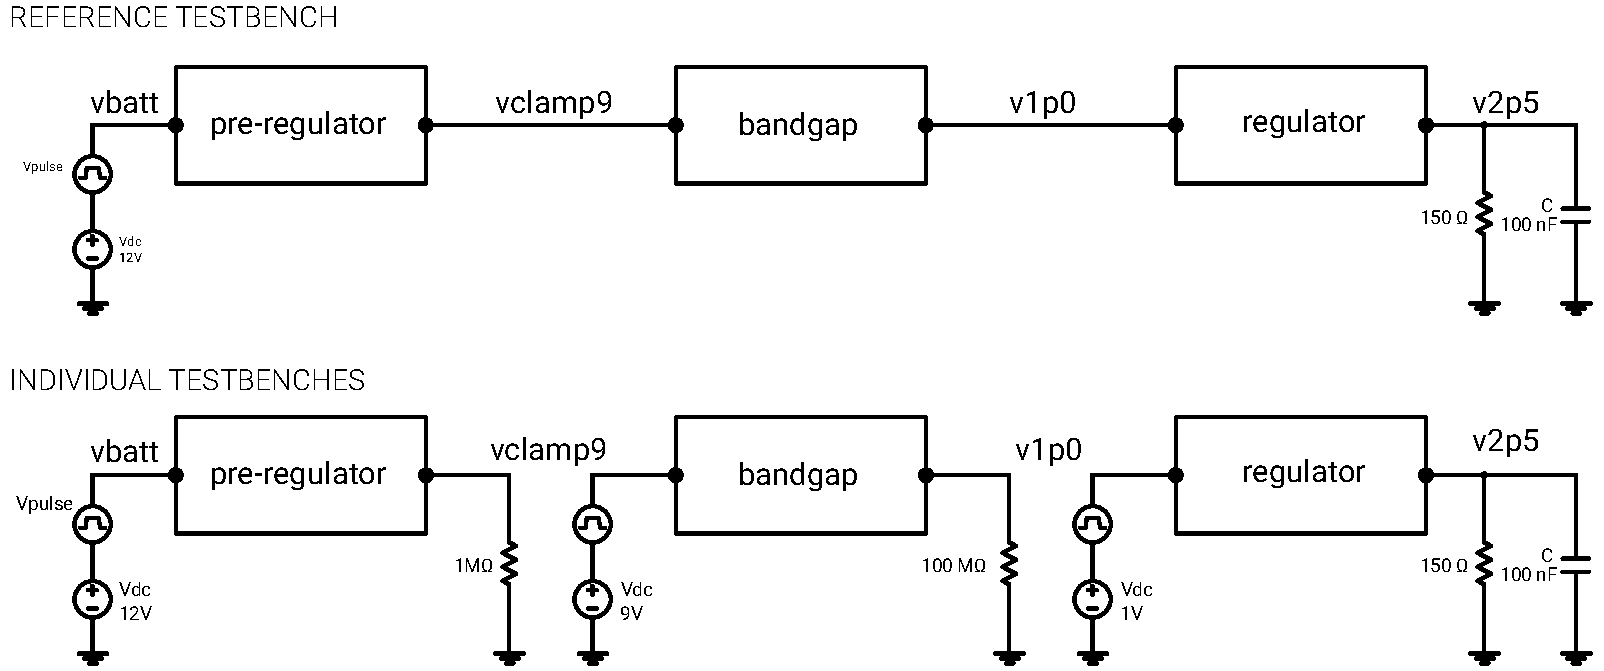
\includegraphics[width=0.98\textwidth]{src/1/figures/hypothesis_testing_setup.pdf}
  \caption{Testbenches used for characterization and hypothesis testing}
  \label{fig:hypothesis-setup}
\end{figure}

% Then do the same thing but with the individual models
La courbe du pré-régulateur seul est donnée Fig. \ref{fig:sim-compare-block1} et comparée avec la simulation totale.
Les deux courbes sont plutôt similaires.
La sortie est estimée avoir une amplitude maximale de -1.5 V (les stress sont d'amplitude négative) et une durée de 880 ns.
Ces deux valeurs sont utilisées comme paramètres d'entrée sur le second modèle, celui du bandgap.

\begin{figure}[!h]
  \centering
  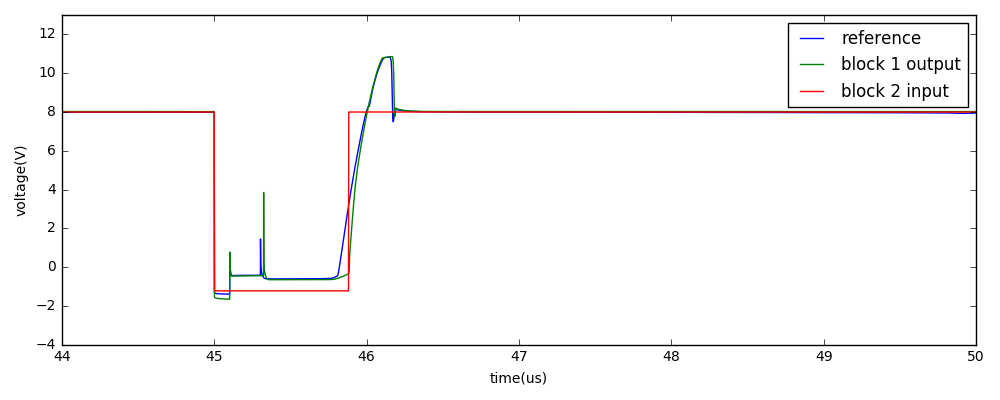
\includegraphics[width=0.98\textwidth]{src/1/figures/simulation_comparison_block1.png}
  \caption{$V_{clamp9}$ waveform}
  \label{fig:sim-compare-block1}
\end{figure}

% Second block output
A la sortie du second block, des différences plus larges apparaissent entre la simulation individuelle et totale. (Fig. \ref{fig:sim-compare-block2}).
La courbe verte a une pente plus longue que la référence.
Néanmoins, les courbes ont quand même des charactéristiques communes en terme d'amplitude maximale et de durée, ce qui est intéressant en regard de cette méthode de modélisation.
La courbe de sortie est analysée et son amplitude maximale déterminée à 0V avec une durée de 2 \textmugreek{}s.
Ces deux valeurs sont appliquées sur l'entrée de la troisième simulation.

\begin{figure}[!h]
  \centering
  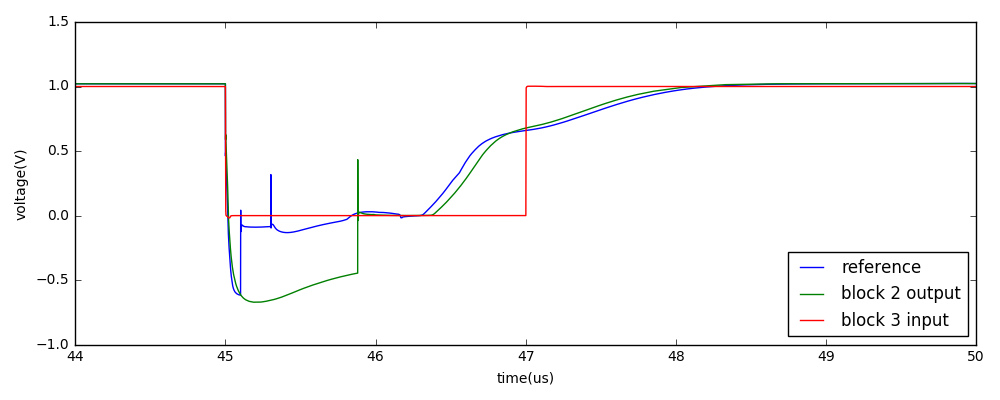
\includegraphics[width=0.98\textwidth]{src/1/figures/simulation_comparison_block2.png}
  \caption{$V_{1p0}$ waveform}
  \label{fig:sim-compare-block2}
\end{figure}

% Third output
A la sortie du dernier bloc, (Fig. \ref{fig:sim-compare-block3}), les deux formes d'onde sont similaires.
La différence d'amplitude maximale est due à un offset aussi présent en statique, et pouvant donc être aisément corrigé.
La courbe de référence est retardée par rapport à la courbe individuelle, mais sinon les deux courbes se ressemblent énormément.

\begin{figure}[!h]
  \centering
  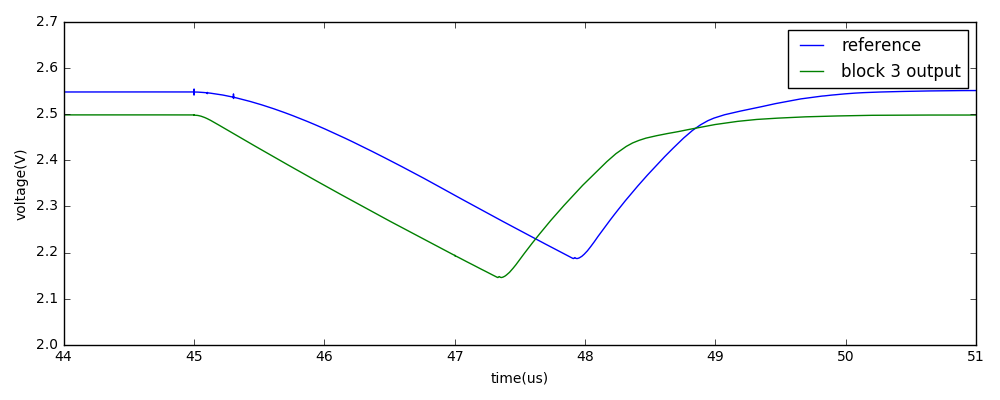
\includegraphics[width=0.98\textwidth]{src/1/figures/simulation_comparison_block3.png}
  \caption{$V_{2p5}$ waveform}
  \label{fig:sim-compare-block3}
\end{figure}

% Conclusion, it works for this case
En conclusion, pour ce cas d'étude, la méthode de simulation et modélisation individuelle aurait permit, par chainage des modèles d'estimer correctement la perturbation sur le bloc de sortie.
Avant de pouvoir généraliser son utilisation, il serait nécessaire de tester cette méthode sur une plus large gamme d'applications.
Elle montre néanmoins des résultats prometteurs.

\section{Méthode boite noire}

% Difference with bottom-up, not the same application, not the same goal
The black-box modeling method relies on the same core principles than the bottom-up modeling approach.
It studies the relationship and transfert function between the input and the output of a silicon function.
Unlike the bottom-up method though, the model is only built for external input and output pins.
It is not meant to be chained with other models, using a special chaining method.
Instead, it targets electrical, board-level circuit simulations.
Basically, the black box model is intented to act as a drop-in replacement for the complete \gls{ic} circuit, for board-level simulations.

% introduction, failure relation between input and output
The main benefit of this model is to abstract the internal silicon complexity.
The model focuses on describing the failure of an output when an input is stressed.
At board-level, failure criteria can be more easily set from the chip specification.
After setting the failure criteria, the approach is to inject rectangular pulses on an input pin, and record when an output is in fault.


% How is the characterization conducted
Once again, a variable width/variable amplitude rectangular pulses are applied on an input pin.
The output pin is then observed to detect for which input parameters it is going out of specification.

% What is characterized
This characterization is performed on the testchip, on the complete regulation function.
The characterization pulses are injected on the $V_{batt}$ input.
The output pin is $V_{2p5}$, the regulated supply.
It is supposed to deliver a 2.5V regulated supply.
The failure criteria is set at a voltage below 2.1V.
It corresponds to a level below which digital cells powered by this supply will have noise margins too small for proper operation.

% Fig X shows the waveform of the VBAT injected current when stressed with a TLP (square) impulse.
% The TLP waveform before the capacitor is shown for reference.
%TODO: WAVEFORM CURRENT VBAT AND TLP BEFORE INJECTION CAPACITOR ?

% Detail the characterization
The characterization table is plotted in Fig. \ref{fig:cz-black-box}.
X-axis is the pulse width, and y-axis is the minimal stress amplitude that caused a failure on the output.

\begin{figure}[!h]
  \centering
  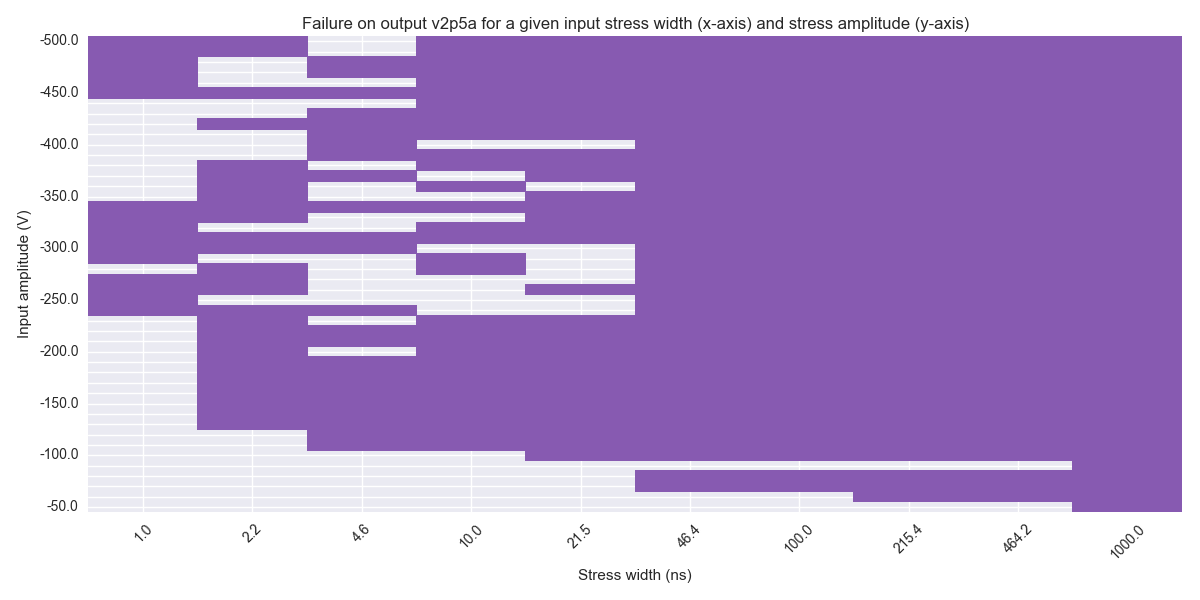
\includegraphics[width=\textwidth]{src/1/figures/black_box_regulator.png}
  \caption{Black-box characterization of the regulation function}
  \label{fig:cz-black-box}
\end{figure}

% What to do with that
%TODO: We that below this value the function is in fail, etc
However, the motivation for this model is to replace the transistor-level schematic inside a SPICE simulation at board-level.
Given a pulse width and an amplitude on $V_{batt}$, the model can estimate the disturbance amplitude and width on $V_{2p5}$.
However, the model itself is not an electrical model, only a failure model.
It cannot determinate, given for instance an input voltage, how much current is flowing into it.
This is also true for the output.
Thus, this method calls for an electrical model of \gls{io}.

\gls{tlp} characterizations are performed on the testchip's regulation function, in powered and unpowered conditions.
For powered conditions, it is considered that full functionality and performance does not matter, just the equivalent impedance of the input or output.
As a consequence, the function is biased but external devices are not connected.
Unpowered and powered characterizations are compared respectively in Fig. \ref{fig:tlp-input-cz} and \ref{fig:tlp-output-cz}.

\begin{figure}[!h]
  \centering
  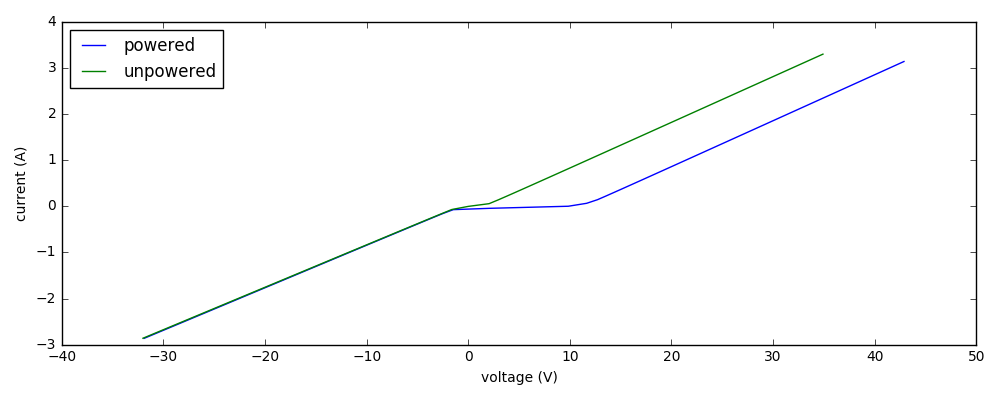
\includegraphics[width=\textwidth]{src/1/figures/tlp_input_characterization.png}
  \caption{TLP characterization of function input in powered and unpowered conditions}
  \label{fig:tlp-input-cz}
\end{figure}

\begin{figure}[!h]
  \centering
  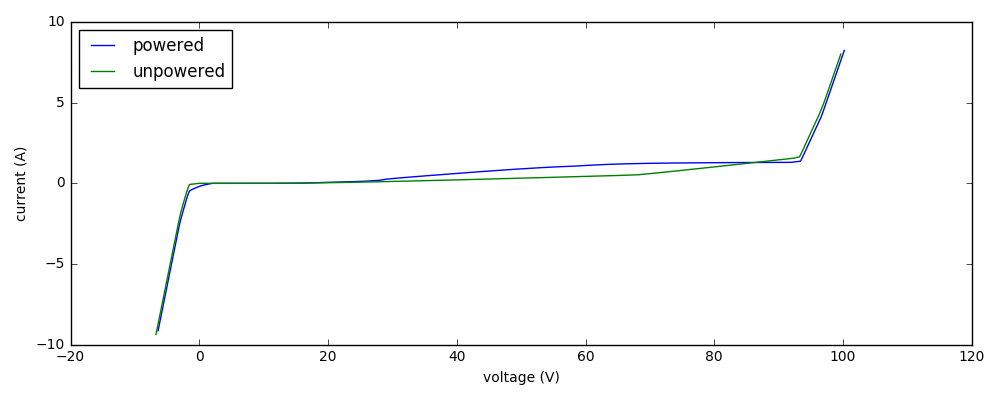
\includegraphics[width=\textwidth]{src/1/figures/tlp_output_characterization.png}
  \caption{TLP characterization of function output in powered and unpowered conditions}
  \label{fig:tlp-output-cz}
\end{figure}


For both input and output ports, large differences are observed between powered and unpowered modes.
Different amount of current are absorbed by the device in each conditions.
Since the model is intended for powered-on simulations, the characterization in powered conditions is chosen.

% Explain the PWL model
The second step of the modelling method is to build an electrically simulatable model of the function.
A piecewise linear model seems well suited for this situation.


% Validate the model with TLP
The verilog-a model is first tested against the complete schematic for the function's input.
After issues described previously were solved, good agreement is achieved between model and complete circuit.
This was verified at -10V, 20V and 40V TLP amplitude (Fig. \ref{fig:compare-model-simu-m10}, Fig. \ref{fig:compare-model-simu-20}, Fig. \ref{fig:compare-model-simu-40}).
The model is considered mostly valid for the input.

\begin{figure}[!h]
  \centering
  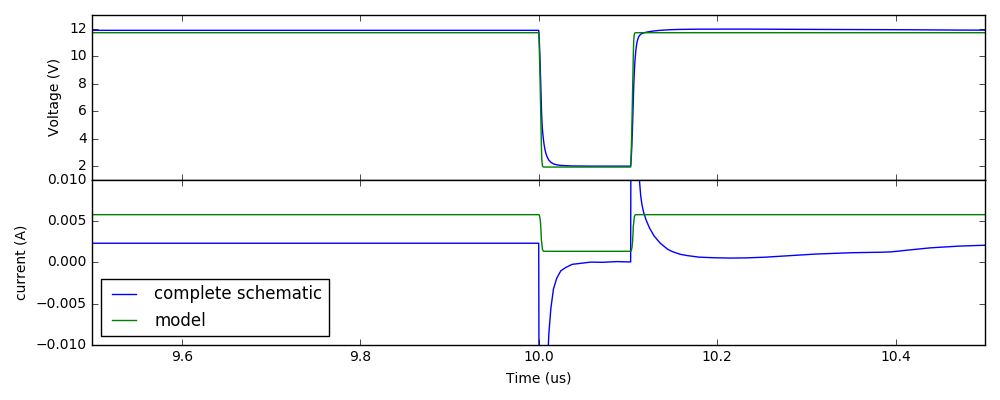
\includegraphics[width=\textwidth]{src/1/figures/comparison_model_total_m10V.png}
  \caption{Comparison of complete schematic and model simulations - -10V TLP}
  \label{fig:compare-model-simu-m10}
\end{figure}


% Check the output
The same test is performed for the function's output model.
The situation is more complex in this case.
The output model must perform three tasks.
First, offer an output impedance close the the one of the real function.
Second, provide a DC value, here corresponding to the regulated 2.5V.
Lastly, reproduce the function reset where the output voltage falls down then restarts.
A first output model is envisionned (Fig. \ref{fig:first-output-model}).

\begin{figure}[!h]
  \centering
  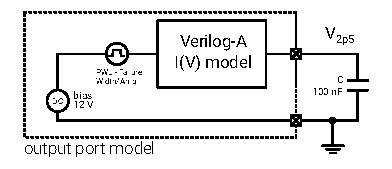
\includegraphics[width=0.3\textwidth]{src/1/figures/first_output_model.png}
  \caption{First proposal for modeling function output}
  \label{fig:first-output-model}
\end{figure}

% Is this first model working
Preliminary and extended tests show that this configuration is not working.

%TODO: Du coup on fait quoi ?


% Conclusion
Black box models of analog integrated functions are very interesting for distributing SPICE models to external parties.
They do not disclose the internal design of the chip, yet they can help achieve system-level ESD simulations.
Ultimately, the goal is to follow the SEED (TODO: Ref) methodology, that indicates that ESD robustness should not be handled at a single level of a system, but at every level (equipment, board, integrated circuit), and that all levels should work efficiently together toward that goal.
Black box models fit very nicely in this methodology.
In this section, a first technique for extracting and creating black-box models was presented.
There is a lot of room for improvements, but it is already working for some intermediate complex cases.
The core principle is that TLP characterization of inputs and ouputs on a biased function is sufficient to extract an equivalent impedance.
This impedance can replace the function in the schematic, during an ESD simulation, in order to reduce complexity and simulation time.
The second core principle is to simplify waveforms into rectangular ones in order to reduce the complexity of the problem.

% Opening work
There are many new leads to explore on these black box models.
First, behavior of the models against more time-varying disturbances such as ESD gun waveforms should be investigated.
Also, the piecewise-linear models should be improved to be more stable, and to fit more closely the extracted I(V) curve.
This technique should be applied to a wider number of analog functions, to observe if it can be used in a general manner.
For now, input and outputs must be simulated separately.
First, the input is simulated, then analyzed to extract the width and amplitude of the disturbance.
This data is then used to configure the output failure source pulse.
The model must be improved in order for the output to react in real-time to the disturbance of the input.
Ultimately, this calls for a Verilog-A model of the failure for instance, plus most likely an improved characterization method able to extract and describe this real-time behavior.

\chapter{Conclusion}

Les décharges électrostatiques sont une source majeure de stress pour les composants électroniques.
Ce stress peut se traduire par une casse matérielle, et ce type de problème est le plus largement étudié dans le domaine des ESD.
Récemment, une nouvelle catégorie de défaillances est apparue appelée défaillance fonctionnelle.
Elles se traduisent par une perturbation temporaire des systèmes électroniques à la suite d'une décharge.
C'est d'autant plus problématique que de nos jours les systèmes électroniques ont des responsabilités accrues vis à vis de notre sécurité.

% Chap 1
Dans le chapitre 1, un état de l'art sur les moyen de tests ESD a été présenté.
Il permet d'identifier les sources classiques de perturbation.
Puis, des outils d'observation et des méthodes de modélisation de fautes ont été détaillés.

% Chap 2
Le chapitre 2 est focalisé sur une méthode de modélisation des systèmes électroniques pour l'ESD.
Une approche modulaire a été favorisée, afin d'avoir des composants réutilisables en vues de modéliser des systèmes complexes.
Un générateur TLP a été modélisé en utilisant cette approche.
% TLP-HMM
Puis, l'expérience acquise via cette étude a permis de développer un nouveau type de générateur HMM basé sur un TLP.
Il offre plusieurs avantages par rapport à un générateur classique, mais requiert encore de multiples améliorations.
% Near-field current processing
Enfin, une méthode de traitement des sondes de champ proche sur puce a été présentée.
Le programme de traitement des données a été libéré \cite{} sous une licence open-source afin de favoriser des améliorations futures.
Deux méthodes différentes furent proposées pour reconstituer la forme originale du courant.

% Chap 3
Le chapitre 3 présente un cas d'étude de défaillance, où une fonction de régulation redémarre à cause d'un ESD.
Le cas de défaillance est étudié, puis un véhicule de test est développé afin d'acquérir plus de données.
Il contient la fonction analogique en question, ainsi que de multiples structures dédiées à sa surveillance et à des mesures.
Malheureusement, des problèmes liés au système de communication du véhicule de test ont empêché d'exploité correctement cette puce.
Des corrections futures devraient permettent de résoudre ce problème.

% Chapter 4
Enfin, le chapitre 4 est focalisé sur le développement d'outils de simulation pour la prédiction de défauts fonctionnels.
Les outils de simulation permettent d'identifier des problèmes très tôt dans le flot de conception, et sont donc extrêmement intéressants.
La principale difficulté pour les ESD au niveau circuit-intégré est la complexité des circuits.
Les problèmes de convergence sont très courants et parfois difficiles à éviter.
La complexité des circuits rends l'investigation assez laborieuse.

% First modelling method
La première méthode est à destination des concepteurs de circuits-intégrés.
Elle consiste à caractériser individuellement en simulation des blocs dans la puce.
La caractérisation est effectuée entre une broche d'entrée et de sortie, à l'aide de signaux impulsionnels rectangulaires.
Puis, ces modèles comportementaux sont connectés ensemble et permettent de propager une perturbation, pour déterminer ses variations globales en terme d'amplitude et de durée.
Cette approche a été testé avec de bons résultats sur le même cas d'étude que celui fabriqué sur silicium.
Il y a de nombreuses améliorations à apporter, mais cette méthode semble d'ores et déjà prometteuse.

% Second modelling approach
La seconde méthode est à destination des équipementiers.
Elle cherche à construire un modèle boite-noire des circuits intégrés, entre une broche d'entrée externe et de sortie externe.
Une fonction de la puce est caractérisée à l'aide encore une fois de signaux rectangulaires impulsionnels, et un modèle boite-noire en est déduit.
Encore à ses débuts, la méthode présente des problèmes pour modéliser des broches fournissant un courant en statique.
Des améliorations futures sont requises pour corriger ces problèmes.

% Final Conclusion
En conclusion, ce travail a permis d'explorer différentes pistes dans ce champ de recherche relativement récent qu'est l'analyse et la prédiction de faiblesses fonctionnelles pour l'ESD.
L'objectif était de fournir des méthodes et outils réutilisables, plutôt que de se focaliser sur un cas d'étude trop spécifique.
La plupart des méthodes présentées ici restent au stade de prototype, et demandent des améliorations futures, mais peuvent servir de base de travail pour d'autres travaux de recherche.

% End of chapter files listing

\tableofcontents
% Bibliography
\bibliographystyle{unsrt}
\bibliography{../src/refs}

\printindex
% Glossary
\setglossarystyle{altlist}
\printglossary


\end{document}
